\documentclass[14pt,openany]{extbook}
\usepackage[T1]{fontenc}
\usepackage{tgheros}
\renewcommand{\familydefault}{\sfdefault}	
\usepackage{ebgaramond}
\usepackage[T1]{fontenc}
\usepackage{etoolbox}

\usepackage{amsmath, amssymb, amsthm}
\usepackage{graphicx}
\usepackage{hyperref}
\usepackage[nameinlink,capitalise,noabbrev]{cleveref}
\usepackage{enumitem}
\usepackage{forest}
\usepackage{tikz}
\usepackage{caption}
\usepackage{subcaption}
\usepackage{geometry}
\usepackage{url}
\usepackage{fancyhdr}
\usepackage{titlesec}
\usepackage{titling}
\usepackage{microtype}
\usepackage{booktabs}
\usepackage{paracol}

\usetikzlibrary{arrows.meta}
\usetikzlibrary{calc}
\usetikzlibrary{shapes.geometric, decorations.pathreplacing}
\usepackage{listings}
\usepackage{xcolor}
\usepackage{float}
\usepackage{xcolor}
\usepackage{tcolorbox}
\tcbuselibrary{skins, breakable}

\usepackage{pgfplots}
\pgfplotsset{compat=1.18}
\usepackage{tikz-3dplot}
\usepackage{pgfplotstable}


\usetikzlibrary{positioning}

\geometry{margin=1in,top=1.2in,bottom=1.2in,headheight=14pt}
\setlength{\parindent}{0pt}
\linespread{1.15}



\tdplotsetmaincoords{65}{115}

\definecolor{dkgreen}{rgb}{0,0.6,0}
\definecolor{gray}{rgb}{0.5,0.5,0.5}
\definecolor{mauve}{rgb}{0.58,0,0.82}

\definecolor{boxborder}{gray}{0.85}
\definecolor{boxbg}{gray}{0.98}
\definecolor{titlecol}{RGB}{0,0,0}
\definecolor{primary}{RGB}{0,0,0}
\definecolor{secondary}{RGB}{80,80,80}
\definecolor{accent}{RGB}{100,100,100}
\definecolor{lightbg}{RGB}{250,250,250}
\definecolor{codebg}{RGB}{245,245,245}

% --- Theorem environments ---
\newtheoremstyle{olympiadplain}%
{6pt}% Space above
{6pt}% Space below
{\itshape}% Body font
{}% Indent
{\color{primary}\bfseries}% Theorem head font
{.}% Punctuation after theorem head
{0.5em}% Space after theorem head
{}% Theorem head spec

\newtheoremstyle{olympiaddefn}%
{6pt}{6pt}%
{}% Body font (upright)
{}%
{\color{primary}\bfseries}% Head font
{.}{0.5em}%


\newtheoremstyle{upright}% name
  {3pt}% space above
  {3pt}% space below
  {}% body font (upright)
  {}% indent
  {\bfseries}% theorem head font
  {.}% punctuation after theorem head
  { }% space after theorem head
  {}% theorem head spec

\theoremstyle{upright}
\newtheorem{problem}{Problem}
\newtheorem{definition}[problem]{Definition}
\newtheorem{lemma}[problem]{Lemma}
\newtheorem{theorem}[problem]{Theorem}
\newtheorem{exercise}[problem]{Exercise}
\newtheorem{corollary}{Corollary}[section]


\renewenvironment{proof}[1][Proof]{%
	\par\vspace{6pt}\noindent%
	{\itshape\color{primary}#1.}\,%
}{\hfill\textcolor{primary}{$\square$}\par\vspace{6pt}}

\newtcolorbox{problembox}[1][]{
	colback=lightbg,
	colframe=gray!40,
	fonttitle=\bfseries,
	title=#1,
	arc=0pt,
	boxrule=0.5pt,
	left=6pt,
	right=6pt,
	top=6pt,
	bottom=6pt
}

\newtcolorbox{examplebox}[1][]{
	colback=lightbg,
	colframe=gray!40,
	fonttitle=\bfseries,
	title=#1,
	arc=0pt,
	boxrule=0.5pt,
	left=6pt,
	right=6pt,
	top=6pt,
	bottom=6pt
}


\definecolor{codebg}{RGB}{248,248,248}
\definecolor{codeframe}{RGB}{220,220,220}
\definecolor{keyword}{RGB}{0,0,160}
\definecolor{comment}{RGB}{63,127,95}
\definecolor{string}{RGB}{163,21,21}
\definecolor{number}{RGB}{0,128,128}
\definecolor{identifier}{RGB}{0,0,0}

\lstdefinestyle{olympiad}{
	backgroundcolor=\color{codebg},
	basicstyle=\ttfamily\small\color{identifier},
	frame=single,
	rulecolor=\color{secondary!30},
	frameround=tttt,
	showstringspaces=false,
	tabsize=2,
	numbers=left,
	numberstyle=\tiny\color{gray},
	stepnumber=1,
	numbersep=8pt,
	keywordstyle=\color{keyword}\bfseries,
	commentstyle=\color{comment}\itshape,
	stringstyle=\color{string},
	numberstyle=\color{number},
	breaklines=true,
	breakatwhitespace=true,
	captionpos=b,
	keepspaces=true,
	columns=fullflexible,
	xleftmargin=10pt,
	xrightmargin=10pt,
	aboveskip=8pt,
	belowskip=8pt
}

\lstset{style=olympiad,language=C++}

\hypersetup{
	colorlinks=false,
	linkcolor=black,
	urlcolor=black,
	citecolor=black,
	bookmarksopen=true,
	bookmarksopenlevel=2,
	pdfauthor={Papangkorn Apinyanon},
	pdftitle={Advanced Data Structures for Olympiad Programmers},
	pdfsubject={Data Structures and Algorithms}
}

\title{Advanced Data Structures\\for Olympiad Programmers}
\author{Papangkorn Apinyanon}
\date{\today}

\pagestyle{fancy}
\fancyhf{}
\fancyhead[LE,RO]{\thepage}
\fancyhead[RE]{\leftmark}
\fancyhead[LO]{\rightmark}
\fancyfoot[C]{}

\titleformat{\chapter}[display]
{\normalfont\huge\bfseries}
{\chaptertitlename\ \thechapter}{20pt}
{\Huge\filright}
[\vspace{2pt}\titlerule]

\titlespacing*{\chapter}{0pt}{30pt}{20pt}

\titleformat{\section}
{\normalfont\Large\bfseries}
{\thesection}{1em}{}
\titlespacing*{\section}{0pt}{14pt}{10pt}

\titleformat{\subsection}
{\normalfont\large\bfseries}
{\thesubsection}{1em}{}
\titlespacing*{\subsection}{0pt}{12pt}{8pt}

\captionsetup{font=small,labelfont=bf,skip=6pt}
\captionsetup[figure]{name=Fig.}
\captionsetup[table]{name=Table}

\setlist[itemize]{leftmargin=1.5em,itemsep=0.1em,topsep=0.5em}
\setlist[enumerate]{leftmargin=1.5em,itemsep=0.3em,topsep=0.5em}
\setlist[description]{leftmargin=1.5em,itemsep=0.3em,topsep=0.5em}

\begin{document}
\maketitle


\chapter*{}
\thispagestyle{empty}

\vspace*{4cm}
\begin{center}
	\Large\itshape

	``The joy of finding things out is the greatest pleasure there is.''

	\vspace{1cm}

	\normalsize — Richard P. Feynman
\end{center}
\thispagestyle{empty}

\iffalse
	\vspace*{3cm}
	\begin{center}
		\begin{tcolorbox}[
				colback=lightbg,
				colframe=secondary,
				arc=4pt,
				boxrule=1pt,
				width=0.75\textwidth
			]
			\centering
			\Large\itshape\color{primary}
			``The joy of finding things out is the greatest pleasure there is.''

			\vspace{0.5cm}

			\large\color{accent}— Richard P. Feynman
		\end{tcolorbox}
	\end{center}
	\thispagestyle{empty}
\fi

\tableofcontents

\addtocontents{toc}{\protect\vspace{1em}}

\chapter{Introduction}

The \href{https://ioinformatics.org/}{International Olympiad in Informatics (IOI)} is one of five international science olympiads. It is essentially a programming competition. Contestants are required to code in C++, solving three problems each day for two days.

The problems often require elegant mathematical intuition, observation, and/or firm knowledge in data structures and algorithms.

The first IOI was held by UNESCO in Bulgaria in 1989.
To participate in the IOI, one needs to be selected to represent their country. Each country sends four students who compete individually.

The team selection test (TST) process differs for each country; however, most countries' processes share striking similarity.

\section{Spirit of OI Competitions}

Each problem presents a puzzle: modeling it mathematically, reasoning its structure, and devising an efficient solution.

OI competitions are more than technical skill and knowledge; they test one's ability to think systemically and stay focused under the stressful contest room. A huge part of contests is time management. With half an hour left on the clock, would you try to fix a bug hidden in hundreds of lines of code, or cut losses and move on to work on other problems?

The ability to make such choices defines medalists.

\iffalse
	\section{The Pathway}

	Most students begin with national or regional Olympiads, organized by their countries or educational institutions. Outstanding performers from these stages often advance to training camps or selection rounds for international representation.

	\subsection{USA (USACO)}

	All competitors in the U.S. start with the USACO online contests, held roughly four times per year. The contests are open to anyone globally. They are divided into four divisions: Bronze, Silver, Gold, and Platinum.

	Each participant starts in the Bronze division and can be promoted by performing well enough in a contest. The promotion system is automatic.
	Top 25–30 performing students from Platinum division are invited to the training camp.

	\subsection{Thailand}

	\raggedright
	The path starts with a written exam to the POSN camps, which selects roughly 90 students to participate in \emph{Thailand Olympiad in Informatics (TOI)}. The gold and silver medalists from TOI are invited to the training camp, which holds rigorous training and exams to choose the four participants.

	\section{Comparisons with online coding competitions}

	Online coding platforms like \emph{Codeforces} hold excellent coding contests which are vastly useful in training for the IOI; however, there is an important contrast in the nature of tasks.

	Generally, tasks in Codeforces are more ad-hoc and observation heavy, while IOI puts more emphasis on standard data structures and algorithms.
	Moreover, Codeforces does not support two-step or communication task types, which have become a crucial part in the IOI.

	%	\section{Why pursue IOI?}	Apart from the medals, training for IOI helps you develop invaluable mental mapping and discipline of problem solving. Also, you can meet really cool people at the competition!
\fi

\section{Prerequisite}

This book does not aim to be a basic programming book -- readers are expected to have firm knowledge on graph theory; dynamic programming; pointers and memory management; time complexity; standard data structures such as binary heap, balanced binary search tree; and standard algorithms such as Dijkstra's. Essentially, the target audiences are USACO Gold and Platinum level coder -- they are assumed to be proficient in using C programming language and to know the basics of C++ standard template library.

\section{Notation}


On a cartesian plane, the main horizontal axis that is the line $y = 0$ is called the OX axis; O means the origin. The main vertical axis that is the line $x = 0$ is called the OY axis.
Given a point $P = (a, b)$ on the plane, we say that $a$, the distance from the point to OY axis, is the \emph{abscissa} of point P, and we say that $b$, the distance from the point to OX axis, is the \emph{ordinate} of point P.

On a cartesian space, there are axes OX, OY, OZ. The plane containing OX and OY axes we call the OXY plane. The OXZ and OYZ planes are defined similarly. A point $P = (a, b, c)$ on the space has \emph{abscissa} a, \emph{ordinate} b, and \emph{applicate} c. As there is no standard name for the distance to from a point in fourth dimension to the OXYZ space, we call it simply as the fourth coordinate.

When a set of $N$ objects with total order -- such as integers between zero and a billion -- is given. We can provide a function from the each member of the set into unique integer ID from $1$ to $N$. This process we refer to as \emph{discretization}. Other sources may refer to it as \emph{coordinate compression}.

All logarithms are in base-2 unless otherwise stated.


\section{Graph Theory}

\begin{definition}
	A \emph{graph} $G = (V, E)$ consists of a set of \emph{vertices} $V$ and a set of \emph{edges} $E$.
\end{definition}

A graph is also called an undirected simple graph.
We typically denote the order $|V|=N$ and the size $|E|=M$.

\begin{definition}
	Vertices $u$ and $v$ are adjacent in graph $G$ if and only if there exists edge $(u, v)$.
\end{definition}

\begin{definition}
	Vertex $u$ and edge $e$ are incident if $u$ is one of the endpoints of $e$.
\end{definition}

\begin{definition}
	A walk is a list of vertices $v_0, v_1, \dots, v_k$ where each consecutive vertices are adjacent.
\end{definition}

\begin{definition}
	A trail is a walk where no edge is repeated.
\end{definition}

\begin{definition}
	A path is a trail where no vertex is repeated.
\end{definition}

\begin{definition}
	A cycle is a walk where no vertex is repeated, except that the first equal the last.
\end{definition}

\begin{definition}
	A tree can be defined by any of the statements following, as they are equivalent; (i) a minimally connected graph.  (ii) a graph where its size is one less than its order.  (iii) a maximally acyclic graph.
\end{definition}

A tree is a minimal connected graph, for deleting any edge cuts it into two.
A tree is a maximal acyclic graph, for adding any edge makes a cycle.
Given any two different vertices $u, v$ in a tree, there is only one path between the two vertices; we denote this path as u-v path. This property is most important.

\begin{definition}
	A rooted tree T is a tree with a vertex $r$ chosen as root.


	We say that $u$ is an ancestor of $v$ if and only if the r-v path contains u. Consequently $v$ is a descendant of $u$.
	The depth of a vertex $u$ is the number of edges in r-u path.
	We say that $p$ is a parent of $u$ if an edge $(p, u)$ exists and $p$ is an ancestor of $u$.
	The subtree $u$ is the tree induced by only descendants of $u$.
\end{definition}

\begin{definition}
	The lowest common ancestor (LCA) of $u$ and $v$ in a rooted tree is the vertex with maximum depth which contains both $u$ and $v$ in its subtree.
\end{definition}

\begin{definition} \textbf{Tree flattening}
	On a rooted tree where vertices are numbered from $1$ to $N$, running a depth-first-search process starting at the root generates discovery time and exit time of each vertex. The discovery time of a vertex $u$, denoted by \texttt{dfn[u]} or \texttt{tin[u]} is one plus the number of vertices visited before it. The exit time of a vertex $u$, denoted by \texttt{tout[u]}, is discovery time of the vertex added by one less than the number of vertices in its subtree. The discovery time list, \texttt{dfn[]}, is a permutation of $1..N$. Its inverse permutation we call \texttt{nfd[]}; it satisfies \texttt{nfd[dfn[u]] = u} for all vertex u.
\end{definition}

Take any vertex $u$ and consider the interval $[dfn[u], tout[u]]$, the vertices which discovery time belongs in the interval is precisely those in subtree $u$.


\chapter{Tricks, Data Structures, and Algorithms}

\begin{center}
	\Large\itshape\color{secondary}
	Conquering Standard Problems
\end{center}

A “standard task” refers to a task that meets one or more of the following criteria: its solution can be easily found online, it lacks novelty, or it consists of well-known techniques that require no significant insight.

\emph{Most tasks are unoriginal}

\iffalse
	\begin{itemize}
		\item \href{https://codeforces.com/problemset/problem/730/B}{CF730B}, \href{https://oj.uz/problem/view/JOI14_ramen}{JOI14\_ramen}
		\item \href{https://acm.timus.ru/problem.aspx?num=2178}{timus2178}, \href{https://codeforces.com/problemset/problem/526/F}{CF526F}
	\end{itemize}


	\subsection*{Example 1}

	Given a tree with $N$ vertices where each vertex $u$ has a positive integer $A_u$, and $M$ queries $(u_i, v_i)$, print the xor-sum of values on all vertices in the simple path from $u_i$ to $v_i$.

	A simple $O(N)$ solution: root the tree arbitrarily, compute $B[u] =$ xor-sum from root to $u$.
	Then answer each query as $B[u_i] \oplus B[v_i]$.
	A more advanced approach might use Heavy-Light Decomposition to handle such queries in $O((N+M)\lg N)$.

	\subsection*{Example 2}

	\href{https://codeforces.com/contest/19/problem/E}{CF19E} can be solved in $O(N + M)$ using DFS-tree logic, but there exist trivial $O((N+M)\log (N+M))$ solutions such as CDQ, Dynacon, or link-cut tree.
\fi


For almost every task one may see in contest, there are some existing tasks with close relation to it. The more problems one solves in practice, the more likely they are to notice the relation. For example, \href{https://oj.uz/problem/view/IOI24_mosaic}{IOI24\_mosaic} closely resembles \href{https://atcoder.jp/contests/arc107/tasks/arc107_e}{ARC107E}, which predates IOI 2024.

The more advanced tricks and data structures you utilize, the fewer observations you need to make. This chapter introduces you to those.
\section{Fenwick Tree (Binary Indexed Tree)}

\begin{tcolorbox}[colback=white, colframe=gray!40, arc=0pt, boxrule=0.5pt, left=6pt, right=6pt, top=4pt, bottom=4pt]
	\small\itshape
	Efficient point updates and prefix queries in $\mathcal{O}(\log N)$ time.
\end{tcolorbox}

A \textbf{Fenwick Tree} (also called \textbf{Binary Indexed Tree} or \textbf{BIT}) is a data structure that provides efficient methods for:
\begin{itemize}
	\item Point add: add \verb|x| to a single element in an array
	\item Prefix sum query: compute the sum of the first $i$ elements
\end{itemize}

Both operations run in $\mathcal{O}(\log N)$ time, where $N$ is the size of the array. The structure requires only $\mathcal{O}(N)$ space.

\subsection{Intuition}

Consider a standard array $A[1..N]$. A naive prefix query requires $\mathcal{O}(k)$ time by summing elements one by one. To improve this, we can precompute prefix sums: $P[i] = A[1] + A[2] + \dots + A[i]$. This gives $\mathcal{O}(1)$ queries but makes updates $\mathcal{O}(N)$ expensive.

The Fenwick Tree achieves a balance: both operations are $\mathcal{O}(\log N)$ by exploiting the binary representation of indices.

\subsection{Lowbit Operation}

The key operation is \texttt{lowbit(i)}, which returns the value of the least significant set bit of $i$.  For example, \texttt{lowbit(12)} = \texttt{lowbit($1100_2$)} = $100_2$ = 4.

To implement \texttt{lowbit} in constant operation, we should first understand Two's Complement.  In most if not all computers to-day, negative integers are internally stored with Two's complements.  Let us consider a hypothetical four-bit signed integer types.  5 would be represented as $0101$.  What would -5 be?

Since the integer type holds four bits, any overflow is truncated.  That is, if we add $0101$ to $1011$, resulting in $10000$, that high bit cannot be stored, and hence the result is $0000$.  And that is the principle of Two's Complement; any number added to its negative must be zero.  Then, one can see that the binary representation of $-x$ is obtained by flipping all the bits in $x$ then adding one to it.  Now, the \texttt{lowbit} operation is obtained by: lowbit(x) = x \& -x.

\subsection{Structure}

A Fenwick Tree stores at each position $i$ the sum of a range of the original array:
\[
	T[i] = \sum_{j=i-\text{lowbit}(i)+1}^{i} A[j]
\]

This forms a hierarchical decomposition. Each index $i$ is responsible for a range of size \texttt{lowbit(i)}.  See \cref{fig:fenwick-viz}.

\begin{figure}[H]
	\centering
	\begin{subfigure}[t]{0.39\linewidth}
		\centering
		\begin{tikzpicture}[
				font=\sffamily,scale=0.85,
				line cap=round, line join=round
			]
			\def\n{16}

			\tikzset{
				wbox/.style={draw=black, line width=1.1pt},
				wfill/.style={draw=gray, fill=gray},
				wtxt/.style={text=black}
			}

			\draw[wbox, rounded corners=2pt] (1,0) rectangle (2,\n);

			% array cells with 0, and left indices 1..n
			\foreach \i in {1,...,\n} {
					\draw[wbox] (1,i-1) rectangle (2,\i);
					%\node[wtxt] at (0.5,\i-0.5) {0};
					\node[wtxt, anchor=east] at (0.75,\i-0.5) {\i};
				}


			% Fenwick tree bars: tree[i] spans (i-lowbit(i)+1 .. i)
			% x-position depends on log2(lowbit(i)) so equal sizes align in columns.
			\foreach \i in {1,...,\n} {
					\pgfmathtruncatemacro{\lb}{int(Mod(\i,2)==0 ? 2 : 1)} % placeholder; overwritten below
					% compute lowbit by repeated division (pure TeX/pgfmath-friendly)
					\pgfmathtruncatemacro{\t}{\i}
					\pgfmathtruncatemacro{\lb}{1}
					\loop
					\pgfmathtruncatemacro{\m}{Mod(\t,2)}
					\ifnum\m=0
					\pgfmathtruncatemacro{\t}{\t/2}
					\pgfmathtruncatemacro{\lb}{\lb*2}
					\repeat
					% now lb = lowbit(i), and k = log2(lb)
					\pgfmathtruncatemacro{\k}{int(round(ln(\lb)/ln(2)))}

					% column x for this lowbit size
					\pgfmathsetmacro{\xc}{2.90 + 1.5*\k}
					\pgfmathsetmacro{\xL}{\xc-0.5}
					\pgfmathsetmacro{\xR}{\xc+0.5}

					% vertical span: bottom = i-lb, top = i
					\pgfmathsetmacro{\yB}{\i-\lb}
					\pgfmathsetmacro{\yT}{\i}

					\draw[fill=gray,draw=none] (\xL,\yB) rectangle (\xR,\yT);
					\draw[fill=pink,draw=none] (\xL,\yT-1) rectangle (\xR,\yT);
					%\node[wtxt, anchor=west] at (\xR+0.18,0.5*(\yB+\yT)) {0};
					\draw[dotted, line width =0.4pt] (2,\yT - .5) -- (\xL, \yT - .5);
				}
		\end{tikzpicture}	\caption{T[] and A[] relationship}
	\end{subfigure}\hfill
	\begin{subfigure}[t]{0.49\linewidth}
		\centering
		\begin{tikzpicture}[
				node/.style={circle,draw,minimum size=6.5mm,inner sep=0pt,font=\small},
				thinE/.style={line width=0.6pt},
				thickE/.style={line width=2.2pt}
			]

			% ---- parameters ----
			\def\N{16}        % draw nodes 0..N
			\def\xscale{1.5}   % horizontal per popcount
			\def\yscale{0.7} % vertical per index
			\def\U{0}        % highlight query path for this u (set 0 to disable)

			% ---- helper: popcount for up to 16 bits (0..65535) ----
			\newcommand{\PopcSixteen}[1]{%
				int(
				mod(#1,2)
				+ mod(floor(#1/2),2)
				+ mod(floor(#1/4),2)
				+ mod(floor(#1/8),2)
				+ mod(floor(#1/16),2)
				+ mod(floor(#1/32),2)
				+ mod(floor(#1/64),2)
				+ mod(floor(#1/128),2)
				+ mod(floor(#1/256),2)
				+ mod(floor(#1/512),2)
				+ mod(floor(#1/1024),2)
				+ mod(floor(#1/2048),2)
				+ mod(floor(#1/4096),2)
				+ mod(floor(#1/8192),2)
				+ mod(floor(#1/16384),2)
				+ mod(floor(#1/32768),2)
				)
			}
			\newcommand{\LowbitSixteen}[1]{%
				int(
				ifthenelse(mod(#1,2)==1,1,
				ifthenelse(mod(#1,4)==2,2,
				ifthenelse(mod(#1,8)==4,4,
				ifthenelse(mod(#1,16)==8,8,
				ifthenelse(mod(#1,32)==16,16,
				ifthenelse(mod(#1,64)==32,32,
				ifthenelse(mod(#1,128)==64,64,
				ifthenelse(mod(#1,256)==128,128,
				ifthenelse(mod(#1,512)==256,256,
				ifthenelse(mod(#1,1024)==512,512,
				ifthenelse(mod(#1,2048)==1024,1024,
				ifthenelse(mod(#1,4096)==2048,2048,
				ifthenelse(mod(#1,8192)==4096,4096,
				ifthenelse(mod(#1,16384)==8192,8192,
				ifthenelse(mod(#1,32768)==16384,16384,
				0))))))))))))))))
				)
			}

			% ---- place nodes: y = i, x = -popcount(i) (0 bottom-right) ----
			\foreach \i in {0,...,\N}{
					\pgfmathtruncatemacro{\pc}{\PopcSixteen{\i}}
					\node[node] (n\i) at ({-(\pc)*\xscale},{(\i)*\yscale}) {\i};
				}

			% ---- draw parent edges: i -> i-lowbit(i) ----
			\foreach \i in {1,...,\N}{
					\pgfmathtruncatemacro{\lb}{\LowbitSixteen{\i}}
					\pgfmathtruncatemacro{\p}{\i-\lb}
					\draw[thinE] (n\i) -- (n\p);
				}

			\newcount\uu \newcount\pp \newcount\steps
			\uu=\U\relax \steps=0\relax
			\loop\ifnum\uu>0
			\advance\steps by 1\relax
			\ifnum\steps>64 \uu=0\relax\fi % safety
			\pgfmathtruncatemacro{\lb}{\LowbitSixteen{\the\uu}}
			\pp=\numexpr \uu-\lb\relax
			\draw[thickE] (n\the\uu) -- (n\the\pp);
			\uu=\pp
			\repeat
		\end{tikzpicture}
		\caption{Query pathway (0 = stop)}
	\end{subfigure}
	\caption{Fenwick tree for $n=16$.}
	\label{fig:fenwick-viz}
\end{figure}


\subsection{Point Update}

To add value $v$ to position $p$:

\begin{lstlisting}[language=C++]
	void update(int p, int v) {
		while (p <= N) {
			T[p] += v;
			p += lowbit(p);
		}
	}
\end{lstlisting}

The algorithm adds \texttt{v} to \texttt{T[j]} for each j whose responsible range contains j.

\begin{lemma}
	The update algorithm modifies $\mathcal{O}(\log N)$ nodes.
\end{lemma}

\begin{proof}
	Each iteration adds \texttt{lowbit(p)} to $p$, flipping the least significant set bit. The number of set bits in $N$ is at most $\left\lfloor \log_2 N \right\rfloor$, so the loop runs $\mathcal{O}\left(\log N\right)$ times.
\end{proof}

\subsection{Prefix Query}


To compute $\text{query}(k) = \sum_{i=1}^{k} A[i]$:

\begin{lstlisting}[language=C++]
int query(int k) {
    int result = 0;
    while (k > 0) {
        result += T[k];
        k -= lowbit(k);
    }
    return result;
}
\end{lstlisting}

The algorithm climbs down the 'staircase', fetching the sum from those indices along the way.  The ranges that belong to those indices are disjoint.  Consider, \texttt{query(13) = query($1011_2$)}; it visits \texttt{T[13], T[9], T[8]}.  The ranges $[13, 13]$, $[9, 12]$, and $[1, 8]$ are disjoint and exactly cover $[1, 13]$.

\begin{lemma}
	The query algorithm visits $\mathcal{O}\left(\log N\right)$ nodes, and these nodes form a partition of $\left[1, k\right]$ into disjoint intervals.
\end{lemma}

\begin{proof}
	Each iteration of the loop removes the least significant set bit from $k$, so the number of iterations equals the number of set bits in $k$, which is at most $\left\lfloor \log_2 k \right\rfloor$.


\end{proof}


\subsection{Point Query}

Of course, just as one can query [a, b] by [b] - [a - 1], [a, a] is trivial by [a] - [a - 1].  But it is wasteful.  One can halves the computation for this special case.

\begin{lstlisting}
	int getpoint(int i) {
		int res = T[i];
		int z = i - (i & -i);         // start-1 of T[i]'s covered range
		for (i--; i != z; i -= i & -i) res -= T[i];
		return res;
	}
\end{lstlisting}


\subsection{Binary Lifting on Fenwick}

It is often desirable to find the first index \texttt{p} such that $\sum_{i = 1}^pA_i >= W$.  Of course, performing normal binary search together with querying the tree yields $\mathcal{O}\left(N \lg^2N\right)$.  There exists a $\mathcal{O}\left(N \lgN\right)$:

\begin{lstlisting}
	int lower_bound_fw(int W) {
		/* return first p with prefix sum >= W; N + 1 if none */
		for (int k = 1 << __lg(N); k; k >>= 1)
			if (p + k <= N && T[p + k] < W) W -= T[p += k];
		return p + 1;
	}
\end{lstlisting}


\begin{problem}[Inversion Count]
Given an array $A[1..N]$, count the number of pairs $(i, j)$ such that $i < j$ and $A[i] > A[j]$.
\end{problem}

\textbf{Solution}

First, discretize the array so that elements are in range $1 \dots N$.
Process elements from right to left. For each position $i$, query the BIT for the number of elements smaller than $A[i]$ seen so far. Then, add $A[i]$ to the BIT.

\begin{lstlisting}[language=C++]
long long count_inversions(int A[], int N) {
	Discretize(A, N);
	memset(T, 0, sizeof T);
    long long ans = 0;
    for (int i = N; i >= 1; i--) {
        ans += query(A[i] - 1);
        update(A[i], 1);
    }
    return ans;
}
\end{lstlisting}

Time complexity: $\mathcal{O}(N \log N)$.

\section{Segment Tree}

\section{Sprase segment tree}

\section{Copy-on-write segment tree}

\section{Fenwick Tree for Maximum (and Why 2D BIT Fails)}

\begin{tcolorbox}[colback=white, colframe=gray!40, arc=0pt, boxrule=0.5pt, left=6pt, right=6pt, top=4pt, bottom=4pt]
	\small\itshape
	1D BIT works for max, but 2D BIT fails for non-commutative operations.
\end{tcolorbox}

The 1D Fenwick Tree can be adapted to support maximum instead of sum. The key insight is that for additive operations like sum, disjoint interval decomposition works perfectly. However, this breaks down in 2D for non-commutative operations like max or min.

\subsection{Fenwick for Maximum}

The one dimensional Fenwick tree can be adapted to support prefix maximum instead of sum.  This is because max of the disjoint intervals is the max of their union.

\begin{lstlisting}[language=C++]
int query_max(int k) {
    int result = -INF;  // or appropriate minimum value
    while (k > 0) {
        result = max(result, T2[k]);
        k -= lowbit(k);
    }
    return result;
}

void update_max(int p, int v) {
    while (p <= N) {
        T2[p] = max(T2[p], v);
        p += lowbit(p);
    }
}
\end{lstlisting}

Now, it is noteworthy that Fenwicks can be modified to support suffix-sum query instead of prefix-sum.  This is done by having the update function climb downstairs and the query function go up, swapping their paths.  Alternatively, one may wrap the functions with $p = N + 1 - p_0$.


\subsection{Why 2D BIT for Maximum Fails}

A 2D Fenwick Tree is conceptually: a 1D BIT over the $x$-dimension, where each $x$-node contains a 1D BIT over the $y$-dimension.

When querying a prefix $[1, x] \times [1, y]$ (a rectangle from the origin):

\textbf{For sum (additive, commutative)}:
The BIT decomposition gives us rectangles that may overlap. Since addition is commutative and associative, overlap doesn't matter:
\[
	\text{sum}(A + B) = \text{sum}(A) + \text{sum}(B)
\]

\textbf{For max (non-commutative, structure-dependent)}:
The same decomposition creates overlapping rectangles. This causes two problems:
\begin{enumerate}
	\item \textbf{Missing points}: Some points in the query rectangle may not be covered by any BIT rectangle
	\item \textbf{Irregular coverage}: The ``remaining'' parts after subtracting BIT rectangles don't form nice axis-aligned sub-rectangles
\end{enumerate}

\begin{lemma}
	For non-commutative non-associative operations, a query decomposition must be a true partition of the query region into disjoint sub-regions.
\end{lemma}

2D BIT cannot guarantee this for arbitrary rectangles defined by $(1, x)$ and $(1, y)$ corners.

\begin{figure}[H]
	\centering
	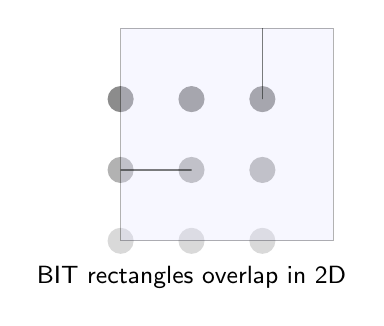
\begin{tikzpicture}[scale=0.9]
		% 2D grid points
		\node (p11) at (0,0) [circle, fill=gray!30, minimum size=0.3cm] {};
		\node (p21) at (1,0) [circle, fill=gray!30, minimum size=0.3cm] {};
		\node (p31) at (2,0) [circle, fill=gray!30, minimum size=0.3cm] {};
		\node (p12) at (0,1) [circle, fill=gray!60, minimum size=0.3cm] {};
		\node (p22) at (1,1) [circle, fill=gray!60, minimum size=0.3cm] {};
		\node (p32) at (2,1) [circle, fill=gray!60, minimum size=0.3cm] {};
		\node (p13) at (0,2) [circle, fill=gray!90, minimum size=0.3cm] {};
		\node (p23) at (1,2) [circle, fill=gray!90, minimum size=0.3cm] {};
		\node (p33) at (2,2) [circle, fill=gray!90, minimum size=0.3cm] {};

		% Query rectangle [1,3] x [1,3]
		\draw[fill=blue!10, opacity=0.3] (0,0) rectangle (3,3);

		% 2D BIT decomposition rectangles (simplified)
		\draw[fill=green!30, opacity=0.5] (0,1) rectangle (1,1);  % BIT node (1,1) covers this
		\draw[fill=green!30, opacity=0.5] (1,2) rectangle (1,2);  % BIT node (1,2) covers this
		\draw[fill=green!30, opacity=0.5] (2,2) rectangle (2,3);  % BIT node (2,2) covers this

		\node[below=0.2cm of p23] (label) at (1,0) {\small BIT rectangles overlap in 2D};
	\end{tikzpicture}
	\caption{2D BIT creates overlapping rectangles}
\end{figure}

\begin{lemma}
	For non-commutative non-associative operations, a query decomposition must be a true partition of the query region into disjoint sub-regions.
\end{lemma}

2D BIT cannot guarantee this for arbitrary rectangles defined by $(1, x)$ and $(1, y)$ corners.

\subsection{Working Alternatives for 2D Max Queries}

\begin{itemize}
	\item \textbf{2D Segment Tree}: $\mathcal{O}(\log^2 N)$ query, $\mathcal{O}(\log^2 N)$ update. Recursively traverse the $x$-tree, and for each relevant node, query the $y$-BIT for maximum.
	\item \textbf{Sqrt Decomposition}: Each $x$-node stores a BIT over $y$. For large ranges, combine precomputed values.
	\item \textbf{Segment Tree of Segment Trees}: A segment tree over $x$ where each node is a segment tree over $y$.
\end{itemize}

\begin{table}[H]
	\centering
	\begin{tabular}{lccc}
		\toprule
		Structure          & Query Time                     & Update Time             \\
		\midrule
		2D BIT (sum)       & $\mathcal{O}(\log^2 N)$        & $\mathcal{O}(\log^2 N)$ \\
		2D BIT (max)       & Fails                          & Fails                   \\
		2D Segment Tree    & $\mathcal{O}(\log^2 N)$        & $\mathcal{O}(\log^2 N)$ \\
		Sqrt Decomposition & $\mathcal{O}(\sqrt{N} \log N)$ & $\mathcal{O}(\log N)$   \\
		\bottomrule
	\end{tabular}
	\caption{2D range query data structures}
\end{table}

\section{Merge small to large}

\begin{problem}[CSES Distinct Color]
On a tree rooted at node $1$ where each node $u$ has its color $C_u$, find for each subtree the number of distinct colors in it.
\end{problem}

\textbf{Solution}

Run a depth-first-search, for each node $u$ we maintain an instance of \verb|std::set| named $S_u$. At the moment we leave a node $u$, $S_u$ shall contain all the colors in its subtree.

We say that a child $v$ of $u$ is heavy if and only if the size of subtree $v$ is at least half the size of subtree $u$. A child $v$ of $u$ is light if it is not heavy. A node either have zero or one heavy child. On our \texttt{DFS(u)} process, once we traversed all of its children we do the following to adjust $S_u$ to its desired state: If $u$ has a heavy child $h$, inherit its set -- don't copy the set over, but change the pointer $S_u$ to the set $S_h$ directly -- this can be done by \texttt{S[u].swap(S[h]);} in C++ -- this operation takes constant time. Now for each light child $v$ of $u$, we iterate over everything in $S_v$ and insert them into $S_u$ in a brute-force manner. Lastly, we insert $C_u$ to $S_u$, and note the size of $S_u$ into $answer_u$.

\begin{lemma}
	This solution takes $O(N \lg^2 N)$.
\end{lemma}
\begin{proof}
	The color element generated by each vertex $u$ only gets moved up $O(\lg N)$ time, for each time we move from a light child to its parent the size of subtree in focus increases twofold. Hence, we do $O(N \lg N)$ moves in total. An extra log factor is added by the \texttt{std::set}.
\end{proof}


\begin{problem} [CF600E -- Lomsat Gelral]
Given a tree rooted at 1, with each vertex $u$ is a color $c_u$. We says that a color $c$ dominates subtree $u$ if no color appears has more occurance than $c$ does in that subtree. For each subtree, print the sum of all of its dominating colors.
\end{problem}
\textbf{Solution} Use a \texttt{std::set} of \texttt{(frequency, color)} pair. The set, being a binary search tree, can fetch the highest frequency. Maintain the sum of dominating colors in addition to it. Then apply merge small to large technique.

\section{DSU on tree -- Sack}

This trick is very closely related to \emph{Merge small to large}, and some people use the terms interchangeably; however, there is a striking difference between them: \emph{We need one instance of data structure in Sack, instead of the $N$ instances in Merge small to large}. The general theme is the same --

\begin{tcolorbox}[colback=white, colframe=gray!40, arc=0pt, boxrule=0.5pt, left=6pt, right=6pt, top=4pt, bottom=4pt]
	\small\itshape
	For each subtree, what would the state of a data structure $D$ be if only the vertices in the subtree is in the data structure?
\end{tcolorbox}


\begin{problem} [CSES Distinct Color]
On a tree rooted at node $1$ where each node $u$ has its color $C_u$, find for each subtree the number of distinct colors in it.
\end{problem}

\textcolor{primary}{\textbf{Solution}} First, we assume the colors are integers between $1$ to $N$, discretize them if they are not. We can use a simple array to support these three operations in constant time: add an instance of a color, remove an instance of a color, and count distinct colors. We were forced to use \texttt{std::set} on the Merge small to large solution, for the array would take $O(N)$ memory and we cannot have $N$ instances of it.

However, here is a trick that let us use one instance. We define heavy and light child the same way. Run a depth-first-search \texttt{DFS(u, keep)} where \texttt{keep} is a boolean. When leaving node $u$, the data structure should have already seen the state where only the vertices in subtree $u$ is put in. If \texttt{keep} is true, it shall stays in that state as we leave the node; if \texttt{keep} is false, we shall clear and empty the data structure before we leave the node.

After entering node $u$ in the depth-first-search -- $D$ is at that time empty -- run \texttt{DFS(v, false)} for each of its light child $v$. $D$ is still empty when we are done. Then, run \texttt{DFS(h, true)} if $u$ has a heavy child $h$. The data structure now contains vertices in subtree $h$. We now iterate over all vertices in subtree $u$ that is not in subtree $h$ and insert them into $D$. Precisely at this point we visit the state of $D$ when the vertices in subtree $u$ are exactly those in $D$ -- take note of the answer we want. Then if \texttt{keep} is false in the current depth-first-search call, empty the data structure by removing everything.

Directly performing this trick and using the array as $D$ solves this problem in $O(N \lg N)$.



\begin{lemma}
	This process performs $O(N \lg N)$ \texttt{add} and \texttt{remove} operations on $D$.
\end{lemma}
\begin{proof}
	Fix a vertex $x$. Consider the unique path from $x$ to the root.

	A single vertex $x$ is (re)inserted into $D$ exactly when $x$ lies in a light subtree of some ancestor $u$ while $u$ is being processed. Each time this happens, the size of the currently ``kept'' part of the tree (the heavy child's subtree) at that ancestor is at least twice the size of the light subtree containing $x$. Therefore, moving up along the ancestors where $x$ belongs to a light child, the size of the context into which we merge at least doubles each time. The doubling can occur at most $\lfloor \lg N \rfloor + 1$ times.

	Hence, each vertex participates in $O(\lg N)$ \texttt{add} (and matching \texttt{remove} for the temporary light traversals) operations. Summed over all $N$ vertices, the total number of operations on $D$ is $O(N \lg N)$.
\end{proof}



\begin{problem}
All problems solvable with Merge small to large are solvable with Sack. Refer to previous section for more practice problems.
\end{problem}


\section{Heavy-Light Decomposition}

\textbf{Heavy-Light Decomposition (HLD)} is a technique for breaking a tree into disjoint paths; so that any path query can be expressed as a small number of contiguous segments in an array. It reduces path query problems to array range query one.

\begin{tcolorbox}[colback=white, colframe=gray!40, arc=0pt, boxrule=0.5pt, left=6pt, right=6pt, top=4pt, bottom=4pt]
	\textbf{Motivation.} In many problems we must process queries along paths between two vertices—such as maximum edge weights. Traversing a path directly is too slow for large $N$. HLD helps us look consider only $O(\lg N)$ segments.
\end{tcolorbox}

\begin{tcolorbox}[colback=white, colframe=gray!40, arc=0pt, boxrule=0.5pt, left=6pt, right=6pt, top=4pt, bottom=4pt]
	\textbf{Concept.} For each node, mark the edge to its largest subtree child as \emph{heavy}; all others are \emph{light}.
	Heavy edges form chains that represent dense parts of the tree; all chains end at a leaf node.
	Any root-to-leaf path crosses at most $\lg N$ light edges, for each move from a vertex to its light children halves the size of the active subtree.
\end{tcolorbox}


\begin{center}
	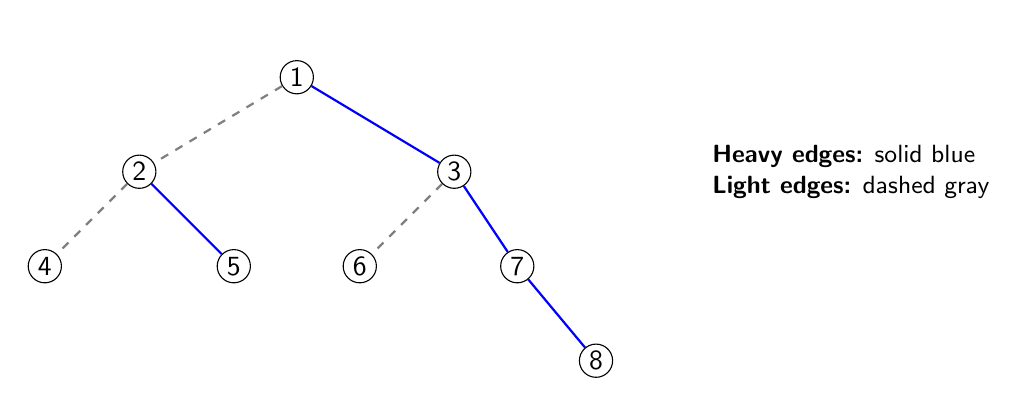
\begin{tikzpicture}[
			every node/.style={circle, draw, inner sep=1pt, minimum size=1.2em},
			edge/.style={thick},
			heavy/.style={edge, blue},
			light/.style={edge, gray, dashed}
		]
		\node (1) at (0,0) {1};
		\node (2) at (-2,-1.2) {2};
		\node (3) at (2,-1.2) {3};
		\node (4) at (-3.2,-2.4) {4};
		\node (5) at (-0.8,-2.4) {5};
		\node (6) at (0.8,-2.4) {6};
		\node (7) at (2.8,-2.4) {7};
		\node (8) at (3.8,-3.6) {8};

		\draw[heavy] (1)--(3);
		\draw[heavy] (3)--(7);
		\draw[heavy] (7)--(8);
		\draw[light] (1)--(2);
		\draw[heavy] (2)--(5);
		\draw[light] (2)--(4);
		\draw[light] (3)--(6);

		\node[draw=none, circle=none, font=\small, align=left, anchor=west] at (5.2,-1.2) {
			\textbf{Heavy edges:} solid blue\\
			\textbf{Light edges:} dashed gray
		};
	\end{tikzpicture}
\end{center}

\textbf{Building the decomposition.}
Compute subtree sizes by DFS. For each vertex, select its child with the largest subtree as heavy.
Nodes connected by heavy edges form a \emph{heavy path}; each path has a \emph{head}.
Linearize the tree by traversing heavy paths consecutively—this allows segment tree indices to correspond to vertex order.

\begin{center}
	\begin{tikzpicture}[
			every node/.style={circle, draw, inner sep=1pt, minimum size=1.2em},
			edge/.style={thick},
			heavy/.style={edge, blue},
			light/.style={edge, gray, dashed}
		]
		\node (1) at (0,0) {1};
		\node (2) at (-2,-1.2) {2};
		\node (3) at (2,-1.2) {3};
		\node (4) at (-3.2,-2.4) {4};
		\node (5) at (-0.8,-2.4) {5};
		\node (6) at (0.8,-2.4) {6};
		\node (7) at (2.8,-2.4) {7};
		\node (8) at (3.8,-3.6) {8};

		\draw[heavy] (1)--(3);
		\draw[heavy] (3)--(7);
		\draw[heavy] (7)--(8);
		\draw[light] (1)--(2);
		\draw[heavy] (2)--(5);
		\draw[light] (2)--(4);
		\draw[light] (3)--(6);

		% DFS order (heavy-first)
		\node[draw=none, fill=none, font=\scriptsize, gray] at (0,0.35) {1};
		\node[draw=none, fill=none, font=\scriptsize, gray] at (2,-0.85) {2};
		\node[draw=none, fill=none, font=\scriptsize, gray] at (2.8,-2.05) {3};
		\node[draw=none, fill=none, font=\scriptsize, gray] at (3.8,-3.35) {4};
		\node[draw=none, fill=none, font=\scriptsize, gray] at (0.8,-2.05) {5};
		\node[draw=none, fill=none, font=\scriptsize, gray] at (-2,-0.85) {6};
		\node[draw=none, fill=none, font=\scriptsize, gray] at (-0.8,-2.05) {7};
		\node[draw=none, fill=none, font=\scriptsize, gray] at (-3.2,-2.05) {8};

		\node[draw=none, circle=none, font=\small, align=left, anchor=west] at (5.2,-1.2) {
			\textbf{DFS order:} heavy-first numbering
		};
	\end{tikzpicture}
\end{center}

\textbf{Path queries.}
To query the path $(u,v)$, repeatedly lift the deeper vertex to the head of its chain, querying each contiguous segment until both vertices lie in the same chain, where a final range query covers the remainder.
Each lift crosses one light edge, hence at most $2 \lg N$ iterations.


\begin{lstlisting}
	vector<int> g[N];
	int sz[N];
	
	void dfs(int u, int p) {
		depth[u] = depth[p] + 1;
		par[u] = p;
		sz[u] = 1;
		for (auto &v: g[u]) if (v != p) {
			dfs(v, u);
			sz[u] += sz[v];
			if (g[u][0] == p or sz[v] > sz[g[u][0]])
				swap(g[u][0], v);
		}
	}
	
	void dfs2(int u, int p, int head_) {
		hld[u] = head_;
		dfn[u] = timer++;
		for (auto &v: g[u]) if (v != p)
		dfs2(v, u);
		out[u] = timer;
	}
\end{lstlisting}

You can also find LCA by the same logic as path query. This is often faster than the binary lift based method.

\begin{lstlisting}
	int lca(int u, int v) {
		while (hld[u] != hld[v]) {
			if (depth[hld[v]] < depth[hld[u]]) swap(u, v);
			v = par[hld[v]];
		}
		return depth[u] > depth[v]? u: v;
	}

	int path_min(int u, int v) {
		int ans = INT_MAX;
		while (hld[u] != hld[v]) {
			if (depth[hld[v]] < depth[hld[u]]) swap(u, v);
			ans = min(ans, /* min of nodes with dfs order
						in range [ dfn[hld[u]], dfn[u] ]
						; can be done with segment tree */);
			v = par[hld[v]];
		}
		ans = min(ans, /* min of nodes with dfs order between
						dfn[u] and dfn[v] */);
		return ans;
	}
\end{lstlisting}


\textbf{K-th ancestor.}

To find $K^{th}$ ancestor, just jump repeatedly until the answer lies in current chain.



\begin{lstlisting}
	int kth(int u, int k) {
		if (k >= depth[u]) return -1;
		while(1) {
			if (depth[u] - depth[hld[u]] >= k)
				return nfd[dfn[u] - k];
			k -= depth[u] - depth[hld[u]] - 1;
			u = par[hld[u]];
		}
	}
\end{lstlisting}


\section{Centroid Decomposition}\label{centroid}

\begin{tcolorbox}[colback=white, colframe=gray!40, arc=0pt, boxrule=0.5pt, left=10pt, right=10pt, top=8pt, bottom=8pt]
	\centering
	\Large\itshape
	Reduce a problem about all paths in the tree to only considering the paths passing through a root.
\end{tcolorbox}
\begin{definition}
	Given a tree of order $N$, a vertex $u$ is a \emph{centroid} if, when $u$ and its incident edges are removed, none of the resulting trees exceeds $N/2$ nodes.
	A tree has one or two centroids.
\end{definition}

\begin{figure}[h!]
	\centering
	\begin{forest}
		for tree={circle,draw,minimum size=1cm,inner sep=1pt,l=1.5cm,s sep=0.7cm}
		[A
			[B
					[C]
					[D]
			]
			[E]
		]
	\end{forest}
	\caption{Example tree -- B is its unique centroid.}
\end{figure}

\subsection*{Finding a Centroid}

To find a centroid of tree $T$, choose arbitrary vertex $a$.
Run a depth-first-search rooted at $a$ to find subtree size of each vertex.
Then repeatedly do following logic: start at $a$, look at children of current vertex,
if any of them have subtree size exceeding half the order of original tree, move to said vertex; else, the current vertex is a centroid.



\subsection*{Centroid Decomposition Algorithm}

Given a tree $T$, we want to find its centroid tree $T+$. To do that, find any centroid $u$ of the tree, this will be the root of $T+$. Remove $u$ from $T$, and for each remaining component, recursively decompose them. Attach the root of resulting trees of their decomposition into $u$.


\begin{lstlisting}
		vector<int> g[N], centree[N];
		int sz[N], dead[N];
		void dfs(int u, int p) {
			sz[u] = 1;
			for (auto v: g[u]) if (!dead[v] && v != p)
				dfs(v, u),
			sz[u] += sz[v];
		}
		int findcen(int u, int p, int treesz) {
			for (auto v: g[u]) if (!dead[v] && v != p && sz[v] * 2 > treesz)
				return findcen(v, u, treesz);
			return u;
		}
		int decom(int u) {
			dfs(u, -1);
			u = findcen(u, -1, sz[u]);
			dead[u] = 1;

			/* we can do a lot of things here ! */

			for (auto v: g[u]) if (! dead[v])
				centree[u].push_back(decom(v));
			return u;
		}
	\end{lstlisting}

\begin{figure}[h!]
	\centering
	\begin{forest}
		for tree={circle,draw,minimum size=1cm,inner sep=1pt,l=1.5cm,s sep=0.7cm}
		[B
			[A,
				[E]]
			[C]
			[D]
		]
	\end{forest}
	\caption{Centroid tree of the example.}
\end{figure}

\subsection*{Key Properties of Centroid Tree}

\begin{lemma}
	The recursion depth of DECOM() -- which is the height of centroid tree -- is $O(\lg N)$.
\end{lemma}
\begin{proof}
	Each recursive call halves the order of focused subgraph.
\end{proof}

\begin{corollary}
	Each vertex in centroid tree has $O(\lg N)$ ancestors.
\end{corollary}

\begin{lemma}
	Sum of subtree size over all vertices is $O(N \lg N)$.
\end{lemma}
\begin{proof}
	A vertex contributes one to size of subtree of each of its ancestors; each vertex contributes at most $\lg N$ to the sum.
\end{proof}

\medskip
The following property is extremely useful when dealing with path information tasks:

Let $T$ be a tree and $T'$ be its centroid tree. Then for all $u$–$v$ paths in $T$, there exists a unique node $\delta(u, v)$ such that the union of $(u, \delta(u,v))$ and $(v, \delta(u,v))$ paths in $T$ is precisely the $u$–$v$ path, and $u$, $v$ belong to subtrees of different children of $\delta(u, v)$ in $T'$. That vertex is precisely the lowest common ancestor of u and v in $T'$.

\medskip
This means each of the $O(N^2)$ possible simple paths is composed of two among the $O(N \lg N)$ paths from vertices to their ancestors in the centroid tree.

\subsection*{Applications}

\begin{problem}
\href{https://dmoj.ca/problem/ioi11p2io}{IOI11\_race}.
Given a tree with weighted edges, find a path such that the sum of its edge weights is exactly $L$.
If multiple paths satisfy this, choose one with the fewest number of edges.
\end{problem}

\smallskip
\textbf{Solution.}
Let the given tree be $T$ and its centroid tree be $T+$.
For each level of decomposition, after we get the centroid $c$, we will consider all path $(u, v)$ satisfying $\delta(u, v) = c$.

\begin{enumerate}[label=\arabic*.]
	\item For each subtree $C_i$ of $c$ (i.e., components after removing $w$), perform a DFS to collect all distances from $c$ to nodes in $C_i$.
	\item Maintain an associative array (e.g. \texttt{std::map}) that records the minimum number of edges required to achieve a given path length from $w$.
	\item For every node $x$ in the current subtree $C_i$,
	      check if there exists a distance $d'$ in the map such that $d + d' = L$, where $d$ is the distance from $x$ to $w$.
	      If such $d'$ exists, update the answer with the sum of corresponding edge counts.
	\item After processing $C_i$, add all its distances and edge counts into the map so that subsequent subtrees can use them.
	\item Clear the map when finishing all subtrees of $w$, and recursively process each $C_i$.
\end{enumerate}

\smallskip
Assuming $L$ is sufficiently small that we can use an array instead of \verb|std::map|, Since each level processes disjoint nodes and each node appears in $O(\lg N)$ decompositions,
the overall complexity is $O(N \lg N)$ — efficient enough for $N \le 2\times10^5$.

\section{Edge Centroid Decomposition}
\label{edge-centroid}

\begin{tcolorbox}[colback=white, colframe=gray!40, arc=0pt, boxrule=0.5pt, left=10pt, right=10pt, top=8pt, bottom=8pt]
	\centering
	\Large\itshape
	Like point centroid, but cooler!
\end{tcolorbox}

In \textbf{standard centroid decomposition}, we recursively remove a vertex whose removal splits the tree into components of size at most half of the original.
In \textbf{edge centroid decomposition}, however, we remove an \emph{edge} instead of a vertex.

\begin{definition}
	An edge $(u, v)$ in a tree $T$ of order $N$ is called an \emph{edge centroid} if, when removed, the sizes of the two resulting subtrees differ as little as possible; equivalently, it minimizes the size of the larger component.
\end{definition}

\begin{figure}[h!]
	\centering
	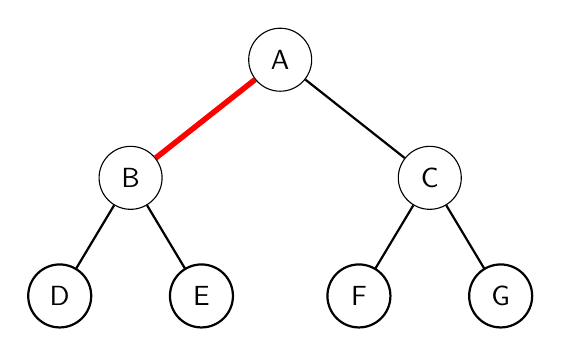
\begin{tikzpicture}[
			every node/.style={circle, draw, minimum size=8mm, inner sep=1pt},
			level 1/.style={sibling distance=38mm},
			level 2/.style={sibling distance=18mm},
			edge from parent/.style={draw, thick}
		]
		\node (A) {A}
		child {node (B) {B}
				child {node (D) {D}}
				child {node (E) {E}}
			}
		child {node (C) {C}
				child {node (F) {F}}
				child {node (G) {G}}
			};

		% highlight centroid edge (A,B)
		\draw[line width=2pt, red] (A) -- (B);
	\end{tikzpicture}
	\caption{Illustration of edge centroid decomposition: the red edge $(A,B)$ is the centroid edge that splits the tree into two balanced (as much as viable) parts.}
\end{figure}

This decomposition defines a recursive structure similar to the centroid tree, but using edges as separators instead of vertices.

\subsection*{Bound on Decomposition Depth}

In vertex-based centroid decomposition, every recursive call processes a tree of size at most $N/2$, ensuring logarithmic recursion depth $O(\lg N)$.

However, this bound does not hold for edge decomposition.
Consider a star graph of order $N$ — removing any edge separates only one leaf from the rest, reducing the size by $1$.
Thus, the recursion depth in worst case is $O(N)$.

\begin{figure}[h!]
	\centering
	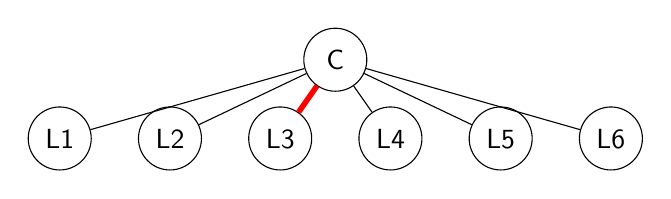
\begin{tikzpicture}[
			every node/.style={circle, draw, minimum size=8mm, inner sep=1pt},
			level distance=1.5cm
		]
		\node (C) {C};
		\foreach \i in {1,...,6} {
				\node (L\i) [below of=C, xshift={( \i - 3.5 )*1.4cm}] {L\i};
				\draw (C) -- (L\i);
			}
		% highlight one edge
		\draw[line width=2pt, red] (C) -- (L3);
	\end{tikzpicture}
	\caption{Star graph}
\end{figure}

\subsection*{Binarizing the Tree}

To ensure balanced splitting, we can \emph{binarize} the tree — i.e. transform every node into a binary structure by inserting auxiliary vertices.
If every node in the resulting tree has degree at most $3$, it can be proven that there exists an edge $(u, v)$ whose removal results in two subtrees, each with size not exceeding $\tfrac{2}{3}N$.

For a formal statement, look up the \emph{Edge-weight Tree Separator Lemma}.

Hence, on a binarized tree, the recursion depth is bounded by:
\[
	O(\log_{1.5} N) = O(\lg N)
\]
This ensures edge centroid decomposition achieves logarithmic height similar to vertex-based decomposition.
\begin{figure}[h!]
	\centering
	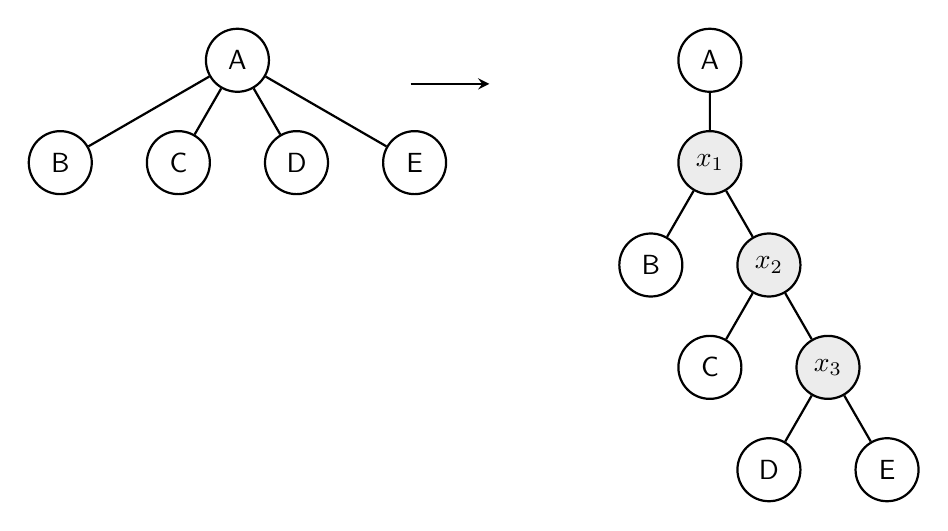
\begin{tikzpicture}[
			every node/.style={circle, draw, minimum size=8mm, inner sep=1pt},
			level distance=1.3cm,
			thick
		]

		% --- Original tree on the left ---
		\node (root1) at (0,0) {A}
		child {node {B}}
		child {node {C}}
		child {node {D}}
		child {node {E}};



		% --- Arrow ---
		\draw[->, thick, >=stealth] (2.2, -0.3) -- (3.2, -0.3);


		% --- Binarized tree on the right ---
		\node (A) at (6,0) {A}
		child {node (x1) [circle, draw, minimum size=8mm, fill=gray!15] {$x_1$}
				child {node {B}}
				child {node (x2) [circle, draw, minimum size=8mm, fill=gray!15] {$x_2$}
						child {node {C}}
						child {node (x3) [circle, draw, minimum size=8mm, fill=gray!15] {$x_3$}
								child {node {D}}
								child {node {E}}
							}
					}
			};

	\end{tikzpicture}
	\caption{Binarizing the tree: replacing a high-degree vertex by auxiliary nodes (gray) to ensure degree $\le 3$.}
\end{figure}


\subsection*{Avoiding Dynamic Data Structures}

Let us revisit \href{https://oj.uz/problem/view/IOI11_race}{\texttt{IOI11\_race}}, discussed in the previous section.

In vertex-centroid decomposition, we often use associative arrays (i.e., std::map) to store the frequency of distances from the centroid.
In the edge-centroid approach, let $(x, y)$ be the current edge centroid; we have only two endpoints.
Thus, we can compute distances from each endpoint separately and use sorted arrays for efficient lookup.

\begin{enumerate}
	\item Compute all distances from $x$ and $y$ to nodes in their subtree to arrays $A$ and $B$ respectively. As the arrays shall be sorted, use breadth-first-search to compute the distances.
	\item Perform monotonic queue trick to find pairs $(a,b)$ such that $a+b=L$.
\end{enumerate}

As the subproblem where we only care about paths passing through the root (i.e. the centroid) is now solved in $O(N)$, the original problem can be solved in $O(N \lg N)$.

\subsection*{Edge Centroid Tree}

In standard centroid decomposition, a vertex in the original tree share label with the corresponding vertex in centroid tree; it works because the centroids are vertices.
As centroids are edges here, it is less straightforward to build a centroid tree.

Say tree $T$ has edge $e = (x, y)$ as its centroid. If $e$ is removed, $T$ will split into $T_x, T_y$ containing $x, y$ respectively. We construct edge centroid tree $T*$ such that $e$ will have a corresponding vertex in the $T*$. Let's denote that node as $\delta(e)$, which is also the root of $T*$. We store following informations in $\delta(e)$: \verb|x, y, leftchild, rightchild|. In addition, of course, any data we wish to store to solve the problem -- as done in standard centroid decomposition. \verb|leftchild|, \verb|rightchild| store the root of $Tx*$ and $Ty*$ respectively. If any of $Tx$ or $Ty$ is a singleton tree, then its corresponding root in $Tx*$ or $Ty*$ need not store any data -- it acts as a dummy vertex.

An advantage of edge centroid tree over standard centroid tree is that each non-dummy vertex has exactly two children. This means we can do \emph{pushup} operation easily.

\begin{problem}
\href{https://codeforces.com/contest/150/problem/E}{CF150E} asks for a simple path with the maximal median edge weight in a weighted tree.
\end{problem}
\textbf{Solution.}
Perform a binary search over the median value.
For threshold $x$, assign each edge weight:
\[
	w'(e) =
	\begin{cases}
		+1, & \text{if } w(e) \ge x, \\
		-1, & \text{otherwise.}
	\end{cases}
\]
Now the task reduces to finding whether there exists a path with nonnegative total $w'(e)$.

\smallskip
Using edge centroid decomposition:
\begin{itemize}
	\item Let $(x, y)$ be the current centroid edge.
	\item Collect distances from $x$’s side into $A[]$, and from $y$’s side into $B[]$.
	\item Instead of sorting, use BFS to fill $A$ and $B$ in nondecreasing order of depth.
	\item Apply a monotonic queue trick to merge $A$ and $B$, avoiding the $\lg N$ factor from segment trees.
\end{itemize}

This yields an $O(N \lg ^ 2 N)$ algorithm with low constants.

%\subsection{Practice Problems}

%\begin{itemize}
%	\item \href{https://www.luogu.com.cn/problem/P3806}{Luogu P3806 – Distance Query o%n Tree}
%	\item \href{https://www.spoj.com/problems/QTREE4/}{SPOJ QTREE4 – Query on Tree IV}
%	\item \href{https://www.spoj.com/problems/QTREE5/}{SPOJ QTREE5 – Query on Tree V}
%\end{itemize}

\section{Cartesian Tree}

A cartesian tree of array $A[1..N]$ , denoted by $C(A)$ is defined as follows: if $A$ is empty, $C(A)$ is the empty tree; else, let $i$ be any $argmax(A)$, we create a vertex labeled $i$ and make it the root of $C(A)$. Then, we assign $C(A_1)$ as the left child of $i$ and $C(A_2)$ when $A_1$ is the prefix of $A$ ending right before $i$ and $A_2$ is the suffix of $A$ starting right after $i$.

Some people use the term \emph{cartesian tree} to mean Treap. In this book the term \emph{cartesian tree} exclusively belongs to what is described in this section and the term \emph{Treap} strictly means the balanced binary search tree.

\begin{figure}[H]
	\centering
	\captionsetup{justification=centering}
	\begin{minipage}{0.9\linewidth}
		\centering
		\setlength{\tabcolsep}{8pt}
		\renewcommand{\arraystretch}{1.2}
		\begin{tabular}{c|ccccc}
			$i$    & 1 & 2 & 3 & 4 & 5 \\
			\hline
			$A[i]$ & 3 & 2 & 5 & 1 & 4
		\end{tabular}

		\vspace{1em}

		\begin{forest}
			for tree={
			draw,
			circle,
			minimum size=10pt,
			inner sep=1pt,
			s sep=10mm,     % sibling distance
			l sep=8mm,      % level distance
			edge={-latex},
			align=center,
			}
			% Cartesian tree of A = [3,2,5,1,4]:
			% root = max (5 at i=3)
			% left subtree from [3,2], right subtree from [1,4]
			[$5 (3)$
			[$3 (1)$
					[NIL, draw=none, minimum size=8pt]
						[$2 (2)$]
				]
				[$4 (5)$
					[$1 (4)$]
						[NIL, draw=none, minimum size=8pt]
				]
			]
		\end{forest}

	\end{minipage}
	\caption{Cartesian tree $C(A)$ for $A=[3,2,5,1,4]$ In parentheses are the corresponding indices in $A$.}
\end{figure}


\subsubsection{Building a Cartesian Tree in $O(N \lg N)$}

Build any data structure which can answer range maximum query over $A$ -- a segment tree works. Then directly implements the recursive building process from the definition of cartesian tree.

\subsubsection{Building a Cartesian Tree in $O(N)$}

Iterate over the array from left to right, maintaining a stack of the right chain of $C(A)$. As we consider $A[i]$, pop the bottom of the right chain so long as it is less than $A[i]$, for $A[i]$ shall not have it as a ancestor. Then insert $A[i]$ into the right chain, linking up pointers as needed.

\begin{lstlisting}
int stk[N], top, k, i,
	rs[N], ls[N]; /* right and left child respectively */
for (int i = 1; i <= n; ++i) {
	k = top;
	while (k > 0 && A[stk[k]] < A[i]) --k;
	if (k) rs[stk[k]] = i;
	if (k < top) ls[i] = stk[k + 1];
	stk[top = ++k] = i;
}
/* the root is at stk[1] */
\end{lstlisting}

\begin{problem}
[CEOI20\_Fancyfence]
\end{problem}


%\section{Persistent Treap}
%(Empty section)

\section{Persistent Segment Tree (copy-on-write)}

In a segment tree of size $N$, we only touches $O(\lg N)$ nodes in \texttt{update} function. $\lg N$ is a small number -- we have the memory to afford making new nodes instead of editing the existing ones (in most case, at least).

Let us do exactly that, the \texttt{update} function take in one root of segment tree, then return a new root, of new version of that segment tree.

We maintain an array \verb|root[0..V]| of pointers to the root for each version, this way we can actually access each version.
Version $0$ is usually the empty tree.

\begin{lstlisting}
struct Node { int lc, rc; long long sum; } t[MAXM];
int root[MAXV], T;  // T = nodes allocated

int update(int v, int l, int r, int pos, int delta){
  int w = ++T;              // new node
  t[w] = t[v];              // copy fields
  t[w].sum += delta;        // this segment contains pos
  if (l == r) return w;
  int m = (l + r) >> 1;
  if (pos <= m)
    t[w].lc = update(t[v].lc, l, m, pos, delta);
  else
    t[w].rc = update(t[v].rc, m+1, r, pos, delta);
  return w;
}
\end{lstlisting}

The \texttt{update} function here still takes $O(\lg N)$ time as in standard segment tree, but each call takes $O(\lg N)$ space. This has tremendous applications, some are described below.

\subsection{Rectangle Sum}
Given $K$ points on cartesian plane, each one with integer weight. You have $Q$ queries to answer; for $i^{th}$ query, print sum of weight of points lying in the rectangle with bottom-left coordinate at $(a_i, b_i)$ and top-left coordinate at $(c_i, d_i)$.

Persistent segtree solves this problem in $O(N \lg N)$ time and space complexity. First we sort the points by their abscissa such that $i < j \implies x_i \le x_j$. Create persistent segment tree representing range sum of weights over the ordinates. The first version is an empty tree. The $i^{th}; i > 1$ version has the contribution of weight of point $j$ for all $j \le i$ at the ordinate $y_j$. To answer a query, find two versions $(E, F)$ such that $E$ is the last version not including any points with abscissa at least $a_i$ and $F$ is the last version not including any points with abscissa more than $c_i$. The answer for $i^{th}$ query then is \texttt{$T_F.query(b_i, d_i) - T_E.query(b_i, d_i)$}. As the difference between the two versions is exactly the segment tree we would get if we only add points having abscissa between $[a_i, c_i]$, the abscissa condition is eliminated by the versioning mechanism, and the ordinate condition is handled by the segment tree range query itself.

\subsection{K-th Order Statistic}

\begin{problem} [SPOJ MKTHNUM]
Given array of integers $A[]$ of length $N$. Answer $Q$ queries -- for $i^{th}$, print the $k_i^{th}$ least element from the subarray $A[l_i..r_i]$.
\end{problem}

First, consider the subproblem where $l_i = 1$. Construct a persistent segment trees where version $i$ is version $i - 1$ added by $1$ at $A[i]$. We can take the tree at version $r_i$ and do walk-on-segtree to find first $z$ such that sum from $(-\infty, z]$ on the segment treeis not less than $k_i$.

Now to solve the full problem, we can think of an imaginary segment tree, where the sum attached to each node is exactly the difference of the corresponding nodes in versions $r_i$ and $l_i - 1$. That is the segment tree we would get if we only add the elements from $[l_i, r_i]$. Now just walk on that segment tree. Since the segment tree is not real, we have to modify our walk function to take in two pointers. Time complexity is $(N \lg N + Q\lg N)$.
Space complexity is $(N \lg N)$.

Given $K$ points on cartesian plane, each one with integer weight. You have $Q$ queries to answer; for $i^{th}$ query, print sum of weight of points lying in the rectangle with bottom-left coordinate at $(a_i, b_i)$ and top-left coordinate at $(c_i, d_i)$.

Persistent segtree solves this problem in $O(N \lg N)$ time and space complexity. First we sort the points by their abscissa such that $i < j \implies x_i \le x_j$. Create persistent segment tree representing range sum of weights over the ordinates. The first version is an empty tree. The $i^{th}; i > 1$ version has the contribution of weight of point $j$ for all $j \le i$ at the ordinate $y_j$. To answer a query, find two versions $(E, F)$ such that $E$ is the last version not including any points with abscissa at least $a_i$ and $F$ is the last version not including any points with abscissa more than $c_i$. The answer for $i^{th}$ query then is \texttt{$T_F.query(b_i, d_i) - T_E.query(b_i, d_i)$}. As the difference between the two versions is exactly the segment tree we would get if we only add points having abscissa between $[a_i, c_i]$, the abscissa condition is eliminated by the versioning mechanism, and the ordinate condition is handled by the segment tree range query itself.

\subsection{Tree Path Range Sum}
\begin{problem} [SPOJ COT]
Given a weighted tree of order $N$ with $Q$ queries -- for each query print $k_i^{th}$ minimum weight on the simple path from $u_i$ to $v_i$.
\end{problem}
\textbf{Solution} Similar to \texttt{MKTHNUM}, make a persistent segment tree where each vertex in a tree has its own version, derived from that of its parent and modified by adding $1$ to the position that is the weight of edge above it. After building it, notice that the segment tree we would get if we only add in the edges in u-v path is exactly the tree we would get by summing up these three version: $T_u + T_v - 2 \cdot T_{lca}$. Walk on segtree again, but this time with three parameters.

\textbf{Extra} How to solve this problem if weights were on the vertices?

\begin{problem}
Given a tree with $N$ vertices, each one having color between $1$ and $N$, and a weight between $1$ to $10^9$. Answer $Q$ queries -- for $i^{th}$ query print the sum of weight of all vertices which lie on the simple path from $u_i$ to $v_i$ and which have color in between $x_i$ and $y_i$.
\end{problem}

\textbf{Solution} This is easier than the previous one, for you do not need to walk on segment tree. Just query the sum and add them up!

\section{Square Root Decomposition: Blocking}


\label{sqr-blocking}

\textbf{Square Root Decomposition (or sqrt-decomposition)} is a classical technique for achieving sublinear query time on static data.
It divides the array into \emph{blocks} of size roughly $\sqrt{N}$ and precomputes aggregated information within each block.

\begin{figure}[h!]
	\centering
	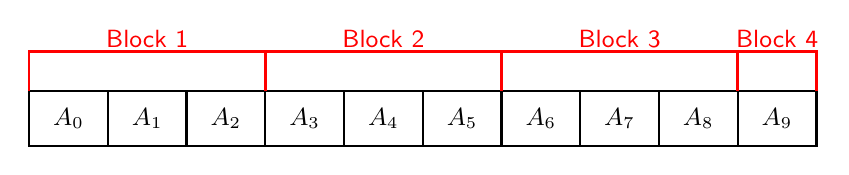
\begin{tikzpicture}[
			thick,
			every node/.style={font=\small, inner sep=1pt},
			block/.style={line width=1pt, red}
		]

		% draw 10 array cells
		\foreach \x in {0,...,9} {
				\draw (\x,0) rectangle ++(1,0.7);
				\node at (\x+0.5,0.35) {$A_{\x}$};
			}

		% draw 4 blocks (sizes: 3, 3, 3, 1)
		\draw[block] (0,0.7) -- (0,1.2) -- (3,1.2) -- (3,0.7);
		\draw[block] (3,0.7) -- (3,1.2) -- (6,1.2) -- (6,0.7);
		\draw[block] (6,0.7) -- (6,1.2) -- (9,1.2) -- (9,0.7);
		\draw[block] (9,0.7) -- (9,1.2) -- (10,1.2) -- (10,0.7);

		% block labels
		\node[above, red] at (1.5,1.2) {Block 1};
		\node[above, red] at (4.5,1.2) {Block 2};
		\node[above, red] at (7.5,1.2) {Block 3};
		\node[above, red] at (9.5,1.2) {Block 4};

	\end{tikzpicture}
	\caption{Blocking}
\end{figure}


Given an array $A[1..N]$, we partition it into blocks of size $B \approx \sqrt N$.
For each block $i$, store a precomputed value, like the minimum of values in the block.

To get minimum over range $[l, r]$: First, find blocks lying completely inside the range and consider their precomputed values. Next, consider all remaining elements in a bruteforce manner; there are at most $2B$ such elements.
This yields $
	O(B + N / B)$ time per query, minimized when $B = \sqrt{N}$.

\section{Square Root Decomposition: Batching}
\label{sqrt-batching}

\textbf{Batching} refers to handling multiple operations at once using square root decomposition — grouping updates or queries into \emph{batches} of size about $\sqrt{N}$, so that each batch can be processed efficiently as a whole.

Whereas blocking divides a data structure \emph{spatially}, batching divides it \emph{temporally}.


Suppose we have $Q$ queries that modify or read the same array.
Instead of updating the array after every single query (which can be slow), we split the $Q$ operations into $\sqrt Q$ batches. Apply all updates within a batch together, and \emph{buffer} new updates.

\begin{problem}
We can maintain an array $A[1..N]$ with $Q$ operations:
\begin{itemize}
	\item \texttt{add(l, r, x)} — add $x$ to every element in range $[l, r]$,
	\item \texttt{get(i)} — query value at position $i$.
\end{itemize}
\end{problem}

\textbf{Solution}

To solve this, we maintain \verb|buffer| -- a list of pending updates.
When a new \verb|add| command comes, put it in \verb|buffer|. If  size of \verb|buffer| reaches $\sqrt Q$, reconstruct the up-to-date version of $A[]$ by using the new updates in \verb|buffer| and difference array -- this is done in $O(N)$ -- then clear \verb|buffer|. To deal with \verb|get(i)| command, take \verb|sum = A[i]|, then for every pending updates which cover \verb|i|, add its value to \verb|sum|. This gives a $O(Q^{1.5} + Q^{0.5}N)$ solution.

\begin{problem}
There is a $N$ by $M$ grid of initially white cells, except one black cell $(s_x,s_y)$.
Then $N\!\cdot\!M-1$ queries $(x_i,y_i)$ are given, each representing a white cell.
For each query, output the Manhattan distance to the nearest black cell and mark that cell as black.
Constraints: $NM\le10^5$.
\end{problem}

\textbf{Solution}


\emph{Naïve idea.}
One could either run a full BFS again after each new black cell is added, or explicitly check all existing black cells for nearest one each time we want the distance.
Both methods require processing all previously updated cells repeatedly, resulting in $O((NM)^2)$ time overall.

\emph{Batching approach.}

\raggedright
Group queries into batches of about $\sqrt{NM}$ in size.
After each batch, perform a multi-source BFS from all black cells so far to get up-to-date distance table.
To get the nearest black cell, look at the current distance table, then consider all the black cells pending in the buffer.
The amortized complexity becomes $O(NM\sqrt{NM})$. This essentially merges the two naive approaches -- a recurring theme in square-root decomposition.
\\

\section{Mo's Algorithm}
\label{sqrt-mo}

\textbf{Mo's Algorithm} is a variant of \emph{blocking}. It trivialize many range query problems, in its most basic form, it groups the queries by chunking one of their endpoint.



\subsection{Basic Mo's -- Subarray query}

\begin{problem}
Distinct color query: Given array $A[1..N]$ of positive integers not exceeding a million. Answer $Q$ queries, where $i^{th}$ query is $l_i, r_i$, print the number of distinct elements in $A[l..r]$. $N \le 100000$ and $Q \le 100000$. Offline processing is allowed.
\end{problem}

% Requires in preamble:
% \usepackage{tikz}
% \usetikzlibrary{calc} % for (A|-B) Manhattan joins

\begin{figure}[ht]
	\centering
	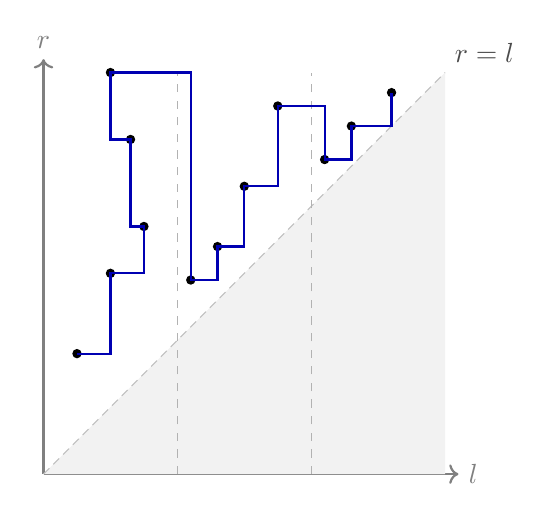
\begin{tikzpicture}[
			scale=0.85,
			axis/.style={->,gray,thick},
			block/.style={gray!60,dashed},
			q/.style={circle,fill=black,inner sep=1.2pt},
			mpath/.style={blue!70!black,thick},
			lbl/.style={font=\scriptsize}
		]

		% Axes and valid region r>=l
		\draw[axis] (0,0)--(6.2,0) node[right]{$l$};
		\draw[axis] (0,0)--(0,6.2) node[above]{$r$};
		\fill[gray!10] (0,0)--(6,0)--(6,6)--cycle;
		\draw[gray!50,densely dashed] (0,0)--(6,6) node[above right,black!70]{$r=l$};

		% Block divisions by l
		\foreach \x in {2,4} \draw[block] (\x,0)--(\x,6);

		% Query points (all satisfy r>=l)
		\coordinate (A0) at (0.5,1.8);
		\coordinate (A1) at (1.0,3.0);
		\coordinate (A2) at (1.5,3.7);
		\coordinate (A10) at (1.3,5);
		\coordinate (A11) at (1,6);
		\coordinate (A3) at (2.2,2.9);
		\coordinate (A4) at (2.6,3.4);
		\coordinate (A5) at (3.0,4.3);
		\coordinate (A6) at (3.5,5.5);
		\coordinate (A7) at (4.2,4.7);
		\coordinate (A8) at (4.6,5.2);
		\coordinate (A9) at (5.2,5.7);

		\foreach \n in {0,...,11} \node[q] at (A\n) {};

		% Manhattan path that stays in r>=l:
		% horizontal to (x_j, y_i), then vertical to (x_j, y_j)
		\draw[mpath]
		(A0) -- (A1|-A0) -- (A1)
		-- (A2|-A1) -- (A2)
		-- (A10|-A2) -- (A10)
		-- (A11|-A10) -- (A11)
		-- (A3|-A11) -- (A3)
		-- (A4|-A3) -- (A4)
		-- (A5|-A4) -- (A5)
		-- (A6|-A5) -- (A6)
		-- (A7|-A6) -- (A7)
		-- (A8|-A7) -- (A8)
		-- (A9|-A8) -- (A9);


	\end{tikzpicture}

	\caption{Mo's algorithm path visualized}
	\label{fig:mo-basic-manhattan}
\end{figure}


\textbf{Solution}
Let us view the problem from a new perspective. Say we have data structure $D$ supporting three operations: add one instance x, remove one instance of x, count distinct number in $D$. This can be implemented in $O(1)$ with an array and a counter.

Now imagine us moving on a cartesian plane where being at $(x, y); x \le y$ means that $D$ contains all the elements from $A[x..y]$ and nothing else. If $D$ is empty, we can be at $(i, i - 1)$ for any $i$. To answer all queries, we need to visit each of $(l_i, r_i)$. We can move from $(x, y)$ to any of the valid 4-adjacent cells in $O(1)$: to move to $(x + 1, y)$, do $D.remove(A[x])$; to move to $(x - 1, y)$, do $D.add(A[x - 1])$; and similar for moving along OY axis. Hence, moving from a point to another takes as many moves as their Manhattan distance.

We want to travel and visit each of the queries $(l_i, r_i)$ with sufficiently small number of moves, for the number of moves is equal to the number of operations we need to perform. The optimal path is hard to find, since that is essentially the Hamiltonian path problem, but we can make a fairly good approximation -- there exists a simple construction giving $O(Q\sqrt N+ N\sqrt N)$ moves.

The construction is as follows: divide the indices ($1..N$) to blocks of size $B$ -- there are $N / B$ such blocks. Bucket the queries by $\lfloor l_i / B \rfloor$. To process a block, move to the first point in the block -- this take at most $2N$ moves. Then, move over the points in increasing order of the ordinate. For each point, we do at most $B$ abscissa moves, and since we only move up and not down, we do at most $N$ ordinate moves for the whole block. There are at most $N / B + 1$ blocks. Hence the total moves is upper bounded by $\frac{N}{B + 1} \cdot (2N + N) + QB$. Let $B$ be $\sqrt N$, then the number of moves -- and time complexity of the solution -- is in $O(N \sqrt N + Q \sqrt N)$.

It seems convoluted, but the implementation is just a custom comparator and moving endpoints around.

\begin{lstlisting}
struct Query {
    int l, r, idx;
    bool operator<(const Query& other) const {
        if (l / B != other.l / B) return l < other.l;
        return r < other.r;
    }
};

const int MAXA = 1'000'000 + 5;
int N, Q, A[MAXN], freq[MAXA], ans[MAXQ];
int distinct = 0, id_ = 0;

auto add = [&](int x) { if (++freq[A[x]] == 1) ++distinct; };
auto remove = [&](int x) { if (--freq[A[x]] == 0) --distinct; };

cin >> N >> Q;
for (int i = 1; i <= N; ++i) cin >> A[i];
vector<Query> q(Q);
for (auto &[l, r, id]: q) cin >> l >> r, id = ++id_;

B = sqrt(N);
sort(q.begin(), q.end());

int L = 1, R = 0;
for (auto [l, r, id] : q) {
    while (L > l) add(--L);
    while (R < r) add(++R);
    while (L < l) remove(L++);
    while (R > r) remove(R--);
    ans[id] = distinct;
}

for (int i = 0; i < Q; ++i)
    cout << ans[i] << '\n';

\end{lstlisting}

\subsubsection*{Parity-based Tiebreaking}

A practical optimization of Mo’s algorithm is to alternate the direction in which queries are ordered inside each block of~$\ell$.
Ordinarily, queries are sorted by block index $\lfloor \ell/B \rfloor$ and then by increasing~$r$,
which causes the right pointer to jump back to the start of the array between blocks.

If even blocks are sorted by increasing~$r$ and odd blocks by decreasing~$r$,
the traversal is likely to be more smooth. This often halves the constant factor of the algorithm on weak testsets.

\begin{figure}[h]
	\centering
	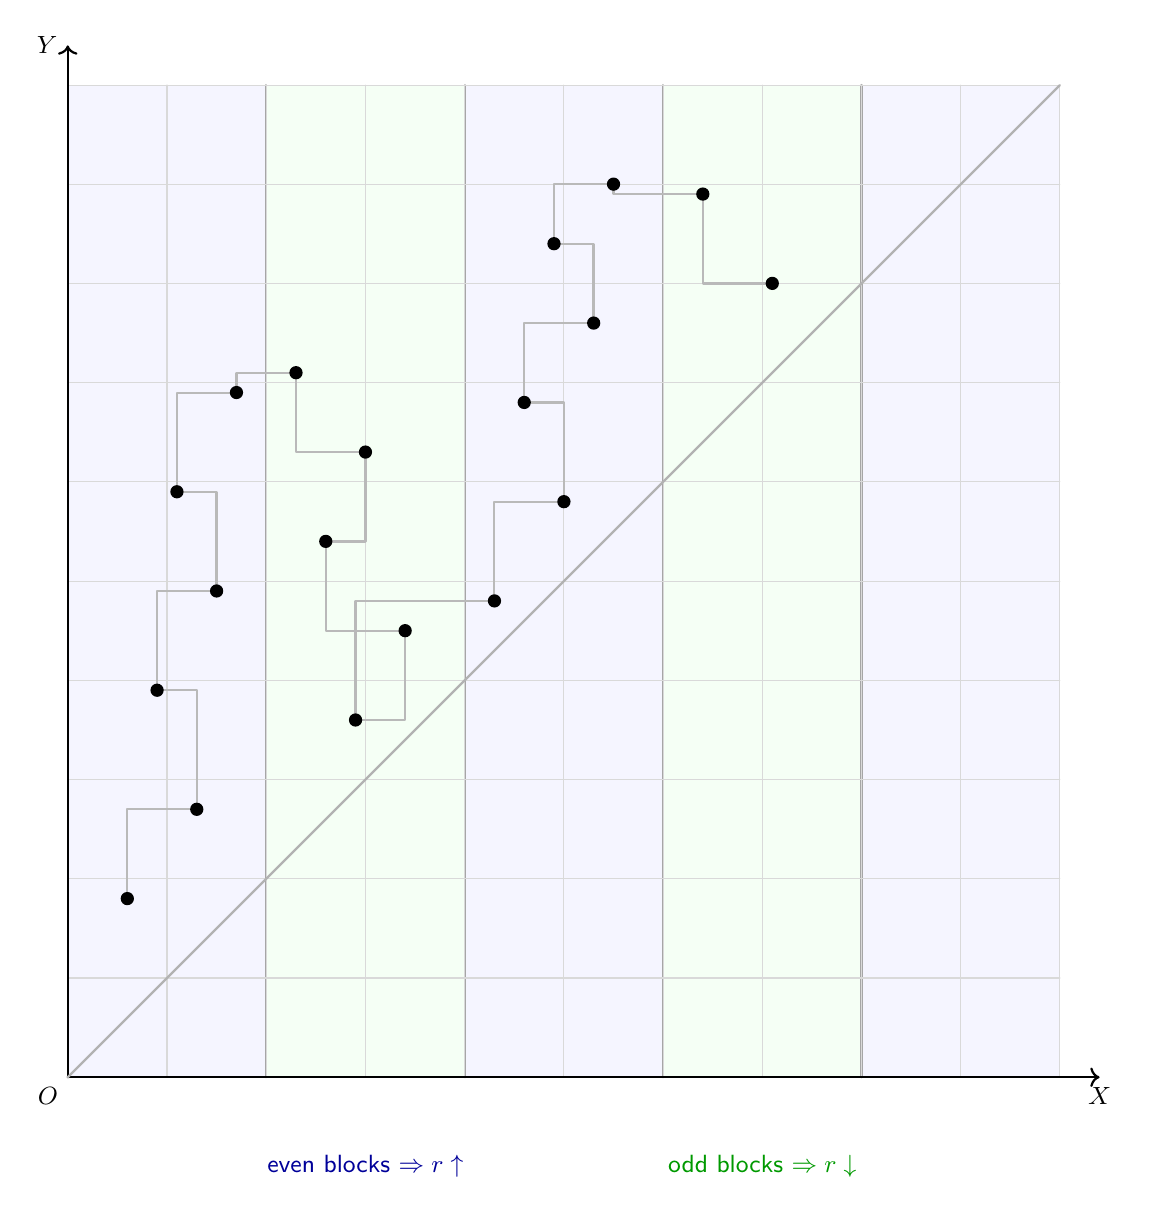
\begin{tikzpicture}[
			scale=1.26,
			line join=round, line cap=round,
			every node/.style={font=\small}
		]
		% Parameters
		\def\N{10}
		\def\B{2}

		% Block shading
		\foreach \k in {0,...,4}{
				\pgfmathparse{mod(\k,2)==0 ? "blue!4" : "green!4"}
				\edef\col{\pgfmathresult}
				\fill[\col] (\k*\B,0) rectangle ++(\B,\N);
			}
		\foreach \x in {0,2,4,6,8}{
				\draw[gray!70, thick] (\x,0) -- (\x,\N);
			}

		% Grid
		\foreach \i in {0,...,\N}{
				\draw[gray!30] (\i,0) -- (\i,\N);
				\draw[gray!30] (0,\i) -- (\N,\i);
			}

		% Axes
		\draw[->, thick] (0,0) -- (\N+0.4,0) node[below] {$X$};
		\draw[->, thick] (0,0) -- (0,\N+0.4) node[left] {$Y$};
		\node[below left] at (0,0) {$O$};

		% Diagonal
		\draw[gray!60, thick] (0,0) -- (\N,\N) node[above right] {};

		% Query coordinates (all above r=l)
		\coordinate (A1) at (0.6,1.8);
		\coordinate (A2) at (1.3,2.7);
		\coordinate (A3) at (0.9,3.9);
		\coordinate (A4) at (1.5,4.9);
		\coordinate (A5) at (1.1,5.9);
		\coordinate (A6) at (1.7,6.9);

		\coordinate (B1) at (2.3,7.1);
		\coordinate (B2) at (3.0,6.3);
		\coordinate (B3) at (2.6,5.4);
		\coordinate (B4) at (3.4,4.5);
		\coordinate (B5) at (2.9,3.6);

		\coordinate (C1) at (4.3,4.8);
		\coordinate (C2) at (5.0,5.8);
		\coordinate (C3) at (4.6,6.8);
		\coordinate (C4) at (5.3,7.6);
		\coordinate (C5) at (4.9,8.4);
		\coordinate (C6) at (5.5,9.0);

		\coordinate (D1) at (6.4,8.9);
		\coordinate (D2) at (7.1,8.0);

		% Manhattan step macro (horizontal then vertical)
		\newcommand{\manhattan}[4]{%
			\draw[gray!55, thick] (#1,#2) -- (#1,#4) -- (#3,#4);
		}

		% Manhattan path between consecutive points
		\manhattan{0.6}{1.8}{1.3}{2.7}
		\manhattan{1.3}{2.7}{0.9}{3.9}
		\manhattan{0.9}{3.9}{1.5}{4.9}
		\manhattan{1.5}{4.9}{1.1}{5.9}
		\manhattan{1.1}{5.9}{1.7}{6.9}

		\manhattan{1.7}{6.9}{2.3}{7.1}
		\manhattan{2.3}{7.1}{3.0}{6.3}
		\manhattan{3.0}{6.3}{2.6}{5.4}
		\manhattan{2.6}{5.4}{3.4}{4.5}
		\manhattan{3.4}{4.5}{2.9}{3.6}

		\manhattan{2.9}{3.6}{4.3}{4.8}
		\manhattan{4.3}{4.8}{5.0}{5.8}
		\manhattan{5.0}{5.8}{4.6}{6.8}
		\manhattan{4.6}{6.8}{5.3}{7.6}
		\manhattan{5.3}{7.6}{4.9}{8.4}
		\manhattan{4.9}{8.4}{5.5}{9.0}

		\manhattan{5.5}{9.0}{6.4}{8.9}
		\manhattan{6.4}{8.9}{7.1}{8.0}

		% Query points
		\foreach \p in {
				A1,A2,A3,A4,A5,A6,
				B1,B2,B3,B4,B5,
				C1,C2,C3,C4,C5,C6,
				D1,D2}{
				\fill[black] (\p) circle (1.9pt);
			}

		% Legend
		\node[blue!60!black] at (3.0,-0.9) {even blocks $\Rightarrow r \uparrow$};
		\node[green!60!black] at (7.0,-0.9) {odd blocks $\Rightarrow r \downarrow$};
	\end{tikzpicture}
	\caption{Parity-based tiebreaking}
\end{figure}


\subsection{Rollback Mo's}

Sometimes, the data structure $D$ might not support deletion -- only rollback. Which means from $(x, y)$ we can either undo the last move, or move to $(x, y + 1)$ and $(x - 1, y)$.

To handle such cases, we use a variant called \emph{Rollback Mo’s algorithm}. The idea is to process queries grouped by their left endpoint block, just as before, but reset the  whole data structure after finishing all queries of one block. Additionally, as rightward moves are not allowed, for each block we starts at the first abscissa to the right of focused block, then temporarily extends to the left and do rollbacks on $D$ to handle the varying left endpoints.

\begin{problem} [JOI14\_Historical] Given array of integers $A[1..N]; 1 \le A[i] \le N$ and $Q$ queries in the form $(l_i, r_i)$. For $i^{th}$ query find $argmax_{x \in \mathbb{Z}}\ x \cdot |\{ j,  A_j = x \}|$.


\end{problem}

\textbf{Solution}
The basic Mo's algorithm with a binary search tree can solve the problem in $O(N^{1.5} \lg N)$; however, it can be solved in $O(N^{1.5})$ with Rollback Mo's. The data structure $D$ here is a frequency array, max value of ($x \cdot \text{frequency of x}$), and the argmax.
We cannot remove an element, for we discard the non-maximum elements. $D$ can be reset in $O(N)$ time. The \verb|add| operation, and its rollback on $D$ take $O(1)$ time.

We solve for each block independently, resetting $D$ afterward. To solve for the block  covering interval $[start, end]$, we starts at the point $(end + 1, end)$, then process the points in that block in increasing order of ordinate -- performing upward moves. We still need to handle the elements in $[l_i, end]$; we do this by performing leftward moves  from $(end + 1, r_i)$ to $(l_i, r_i)$ just before we fetch the answers. After the answer to $i^{th}$ query is obtained, we rollback the changes until we are back at $(end + 1, r_i)$ -- no rightward moves are done here.

\begin{problem}
[SheepDev Round 1 -- C] You are given a graph with N vertices and M edge (parallel edges
and loops are possible).
Each edge has an integer weight not exceeding 1000000000.
The vertices are numbered 0 to N - 1.
You must process Q queries, each in form of pair “x y”. You shall
imagine a situation where every edges with weight less than x or
more than y is removed from the graph, then print the number of
connected component in the graph.
Note that you are only imagining it, and no edges actually get
removed.
\end{problem}

\textbf{Solution}
Sort the edges, then each query is limiting the graph to using only an interval of edges. Use Rollback Mo's with disjoint-set-union to solve it. Time complexity is $O(N^{1.5} \lg N)$.

\subsection{Balancing the Time Complexity}
\label{balancingmo}

\emph{We do $O(Q \sqrt N)$ moves but fetch the answer merely $Q$ times.}

\begin{problem}
Given an array $A$ of length $N$ where each element is a positive integer between $1$ and $N$. For each query $(l_i, r_i)$, determine whether there exists a \textbf{majority element} in the subarray $A[l_i..r_i]$, i.e.\ a value that occurs more than $\frac{r_i - l_i + 1}{2}$ times.
\end{problem}

\textbf{Solution.}

We can achieve $O(N \sqrt N)$ total time. Assume $Q = O(N)$.

Notice that Mo's algorithm executes $O(Q\sqrt N)$ moves but only $Q$ heavy queries, we can afford each query on the data structure to cost $\sqrt N$ times more than the add and remove operations while not affecting the overall complexity.

We apply Mo's algorithm to handle the $(l_i, r_i)$ intervals. As usual, we maintain a frequency array
\[
	\texttt{freq}[x] = |\{ j \in [l, r] \mid A[j] = x \}.
\]

Each movement of the endpoints in Mo's order adds or removes one element, so the total number of \texttt{add()} and \texttt{remove()} operations is $O(N \sqrt N)$.

To check whether a majority element exists in the current range, we need to know whether some frequency exceeds $\frac{r - l + 1}{2}$.
Instead of scanning all values, we maintain a histogram over the current frequency distribution:

\[
	\texttt{bucket}[k] = \text{number of distinct values with frequency exactly } k.
\]

When we add or remove a value $x$, we update its frequency and adjust two counters:

\begin{lstlisting}[language=C++]
void add(int x) {
    int f = freq[x];
    bucket[f]--;             // one fewer element with frequency f
    blockSum[f / B]--;
    ++freq[x];
    ++bucket[freq[x]];
    ++blockSum[freq[x]];
}
\end{lstlisting}

\noindent
where \texttt{blockSum[i]} stores the total number of elements whose frequencies fall in the $i$-th block.

All these operations are $O(1)$.

To answer a query, we simply check whether there exists any $f > \frac{r - l + 1}{2}$ such that $\texttt{bucket}[f] > 0$:
\begin{lstlisting}[language=C++]
bool hasMajority(int len) {
    int threshold = len / 2 + 1;
    int b = threshold / B;
    for (int i = b + 1; i < numBlocks; ++i)
        if (blockSum[i] > 0) reference true;
    for (int f = threshold; f < (b + 1) * B; ++f)
        if (bucket[f] > 0) return true;
    for (int f = threshold; f < min((b + 1) * B, MAXF); ++f)
        if (bucket[f] > 0) return true;
    return false;
}
\end{lstlisting}

The query operation thus costs $O(\sqrt N)$, while updates remain $O(1)$.

\medskip
\noindent
\textbf{Complexity Analysis.}
\[
	O(N \sqrt N) \text{ moves} + Q \cdot O(\sqrt N) \text{ queries } = O((N + Q)\sqrt N).
\]

\iffalse
	\subsection{Balancing the Time Complexity}

	\begin{problem}
	Given an array $A$ of length $N$ where each element is a positive integer between $1$ to $N$, and another array $B$ of length $N$ where $B[i]$ is an integer between one and a billion. There are $Q$ queries, each one is in form $(l_i, r_i, x_i, y_i); 1 \le l_i \le r_i \le N, 1 \le x_i \le y_i \le N$ -- answer for each query the value $max_{x_i \le z \le y_i} (B[z] \cdot |\{ j, l_i \le j \le r_i \land A[j] = z \}|)$.
	\end{problem}

	\textbf{Solution}

	$O(N \sqrt N)$ can be done. Here we assume $Q = O(N)$.

	We utilize Mo's with rollback here. Mo's help us deal with the $(l_i, r_i)$ query interval. The main concern is what we shall use as the underlying data structure to solve the $(x_i, y_i)$ part. Segment tree is one obvious choice; however, it leads to total time complexity of $O(N^{1.5} \lg N)$ which may be too slow. The data structure which we want here must support these operation: \texttt{insert(x)} adds one instance of x, \texttt{query(a, b)} return $max_{a \le z \le b}  (B[z] \cdot \text{frequency of z})$.

	\raggedright
	An important insight here is that Mo's process will call \texttt{insert()}   $O(N \sqrt N)$ times, but it calls \texttt{query()} merely $Q$ times. This means if \texttt{insert()} takes constant time, then \texttt{query()} can take $O(\sqrt N)$ time, and we still have a fast $O(N^{1.5})$ solution.
\fi
The allowed $O(\sqrt N)$ time motivates a square-root decomposition approach. We design the data structure as follows: block the integers from $1$ to $N$ into blocks of size $K$. On $insert(x)$ we calculate value of $x$ as the chosen value -- if that value is the maximum in its block (that is block $\lfloor \frac{x}{K} \rfloor$), we take note of that maximum in the block.
On $query(a, b)$ operation, look at all blocks which lie completely in $[a, b]$, each of their maximum is an lower bound for the answer. Then we look at each index on the border individually, checking if their value is a tighter lower bound. Of course, we let $K = O(\sqrt N)$ to obtain $O(\sqrt N)$ complexity.
\iffalse
	\subsection{Mo's on Tree Path}

	Handling subtree queries with Mo's is trivial -- use tree-flattening and do Mo's on the depth-first-search order.
	Tree paths, however, is tricky. We can

	\begin{exercise} [SPOJ COT2 – Count on a Tree
			II]
	\end{exercise}
\fi
\subsection{3D Mo's}
Standard Mo's algorithm is limited to static arrays. To handle point updates, the algorithm is extended by adding a third dimension: time.


\begin{problem}
Dynamic distinct color query.  Given array $A[1..N]$ of positive integers not exceeding a million. Answer $Q$ command, where $i^{th}$ command can be either \verb|ask(l_i, r_i)|: print the number of distinct elements in $A[l..r]$, or \verb|upd(p_i, x_i)|: change $A[p_i]$ to $x_i$. $N \le 100000$ and $Q \le 100000$. Offline processing is allowed.
\end{problem}


\begin{figure}[h]
	\centering
	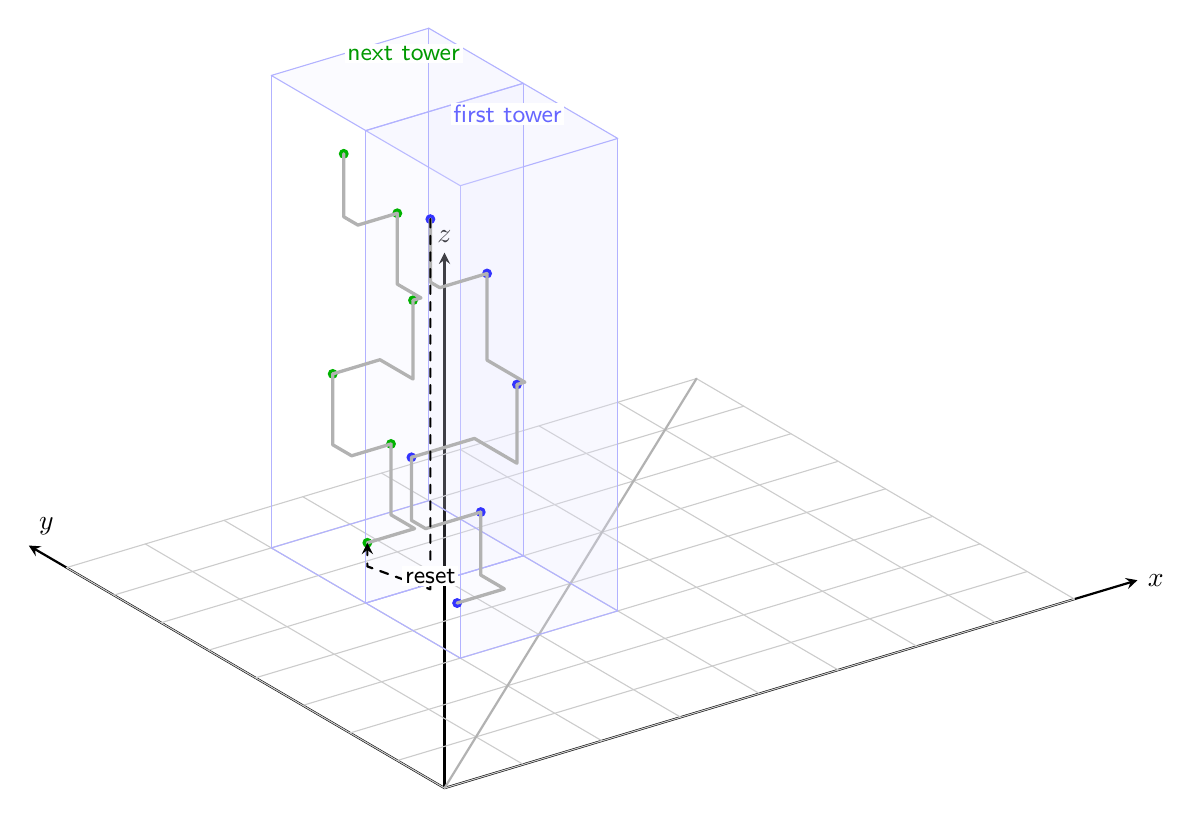
\begin{tikzpicture}[
			% Perspective: viewer looking from above-left
			x={(1cm,0.3cm)},
			y={(-0.6cm,0.35cm)},
			z={(0cm,1cm)},
			line join=round, line cap=round, >=stealth
		]

		% Parameters
		\def\N{8}
		\def\B{2}
		\def\Z{6}

		%-------------------
		% Axes
		%-------------------
		\draw[->, thick] (0,0,0) -- (\N+0.8,0,0) node[anchor=west] {$x$};
		\draw[->, thick] (0,0,0) -- (0,\N+0.8,0) node[anchor=south west] {$y$};
		\draw[->, thick] (0,0,0) -- (0,0,\Z+0.8) node[anchor=south] {$z$};

		%-------------------
		% Base grid (x–y plane)
		%-------------------
		\foreach \i in {0,...,\N} {
				\draw[gray!40, thin] (\i,0,0) -- (\i,\N,0);
				\draw[gray!40, thin] (0,\i,0) -- (\N,\i,0);
			}
		\draw[gray!60, line width=0.8pt] (0,0,0) -- (\N,\N,0);

		%-------------------
		% Tower macro
		%-------------------
		\newcommand{\tower}[4]{% x0,y0,B,H
			\coordinate (A) at (#1,#2,0);
			\coordinate (B) at (#1+#3,#2,0);
			\coordinate (C) at (#1+#3,#2+#3,0);
			\coordinate (D) at (#1,#2+#3,0);
			\coordinate (A') at (#1,#2,#4);
			\coordinate (B') at (#1+#3,#2,#4);
			\coordinate (C') at (#1+#3,#2+#3,#4);
			\coordinate (D') at (#1,#2+#3,#4);

			% transparent faces (behind grid)
			\fill[blue!10, opacity=0.15] (A)--(B)--(B')--(A')--cycle;
			\fill[blue!10, opacity=0.15] (B)--(C)--(C')--(B')--cycle;
			\fill[blue!10, opacity=0.15] (A')--(B')--(C')--(D')--cycle;

			% outlines
			\draw[blue!30, thin] (A)--(B)--(C)--(D)--cycle;
			\draw[blue!30, thin] (A')--(B')--(C')--(D')--cycle;
			\foreach \p/\q in {A/A',B/B',C/C',D/D'}{
					\draw[blue!30, thin] (\p)--(\q);
				}
		}

		% first tower
		\tower{2}{3}{\B}{\Z}
		% second tower directly above (4-adjacent)
		\tower{2}{5}{\B}{\Z}

		%-------------------
		% Path macro
		%-------------------
		\newcommand{\mstep}[6]{%
			\draw[gray!60, very thick]
			(#1,#2,#3) -- (#4,#2,#3) -- (#4,#5,#3) -- (#4,#5,#6);
		}

		%-------------------
		% Query points in first tower (blue)
		%-------------------
		\foreach \x/\y/\z in {
				2.2/3.4/0.5,
				2.8/3.9/1.3,
				2.1/4.2/2.1,
				2.9/3.3/3.1,
				3.0/4.1/4.2,
				2.4/4.3/5.0
			}{
				\fill[blue!80] (\x,\y,\z) circle (1.8pt);
			}

		% Connect them
		\mstep{2.2}{3.4}{0.5}{2.8}{3.9}{1.3}
		\mstep{2.8}{3.9}{1.3}{2.1}{4.2}{2.1}
		\mstep{2.1}{4.2}{2.1}{2.9}{3.3}{3.1}
		\mstep{2.9}{3.3}{3.1}{3.0}{4.1}{4.2}
		\mstep{3.0}{4.1}{4.2}{2.4}{4.3}{5.0}

		%-------------------
		% Query points in next tower (green)
		%-------------------
		\foreach \x/\y/\z in {
				2.2/5.3/0.6,
				2.8/5.8/1.5,
				2.3/6.2/2.4,
				2.9/5.5/3.4,
				3.0/6.0/4.3,
				2.5/6.3/5.1
			}{
				\fill[green!70!black] (\x,\y,\z) circle (1.8pt);
			}

		% Path in next tower
		\mstep{2.2}{5.3}{0.6}{2.8}{5.8}{1.5}
		\mstep{2.8}{5.8}{1.5}{2.3}{6.2}{2.4}
		\mstep{2.3}{6.2}{2.4}{2.9}{5.5}{3.4}
		\mstep{2.9}{5.5}{3.4}{3.0}{6.0}{4.3}
		\mstep{3.0}{6.0}{4.3}{2.5}{6.3}{5.1}

		%-------------------
		% Reset arrow (end exactly at first green point)
		%-------------------
		\draw[dashed, thick, ->]
		(2.4,4.3,5.0) -- (2.4,4.3,0.3) -- (2.2,5.3,0.3) -- (2.2,5.3,0.6);

		\node[fill=white, inner sep=1pt] at (2.7,4.8,0.2) {\small reset};

		%-------------------
		% Labels
		%-------------------
		\node[blue!60, fill=white, inner sep=1pt] at (3.2,4.0,\Z+0.2) {\small first tower};
		\node[green!60!black, fill=white, inner sep=1pt] at (3.2,6.2,\Z+0.2) {\small next tower};

	\end{tikzpicture}

	\caption{
		3D Mo’s algorithm in OXYZ space.
		Each query $(\ell,r,t)$ is represented as a point.
		The OXY plane is partitioned into blocks of size $B\times B$ which extends in OZ axis, forming vertical \emph{towers}.
		Within each tower, enlarged query points are processed along a light-gray path.
	}
\end{figure}

Rather than a cartesian plane, now we imagine a 3D space. The corresponding state of point $(x, y, z)$ is that $D$ contains only the elements from $A[x..y]$ after the $z^{th}$ command.
Moving parallel to OX and OY axes is done the same way as in static distinct color query. To move in the direction of OZ axis, we can add and remove some elements from $D$. There are $O(1)$ such operations we have to do to move one step.

Since we can still move efficiently, it is a matter of finding a short enough path. One way to do that is to divide both the OX and OY axes to blocks of size $B$. We then process each "tower" -- $B \times B$ square which expands infinitely in OZ axis separately; at the start of each tower we reset $D$ -- move it to the point with lowest applicate, then move our state as needed, visiting all points contained in that tower in increasing order of applicate.

The time complexity is $O((N/B)^2 \cdot Q + Q \cdot B)$. That is minimized when $B \approx N^{2/3}$: $O(N^{5/3} + QN^{2/3})$.
If $Q$ is $O(N)$ then it is nicely $O(N^{5/3})$. Guess what the time complexity of 4D Mo's would be!

\begin{problem}
\href{https://www.spoj.com/problems/XXXXXXXX/}{\texttt{SPOJ - XXXXXXXX}}
\end{problem}


%\subsection{Sweepline Mo's -- Offline for the second time}

\subsection{4D Mo's}

\begin{tcolorbox}[colback=white, colframe=gray!40, arc=0pt, boxrule=0.5pt, left=10pt, right=10pt, top=8pt, bottom=8pt]
	\centering
	\Large\itshape
	To deal with a 14-dimensional space, visualize a 3-D space and say 'fourteen' to yourself very loudly. Everyone does it.
	\par\vspace{0.3cm}
	\normalsize — Geoffrey Hinton
\end{tcolorbox}

\begin{problem} [Codeforces 1767F] Given a tree of order $N$ rooted at vertex $1$. Each vertex has integer $v_i$ written on it. Answer $Q$ queries; the $i^{th}$ query is $(u_i, v_i)$. To answer it, you shall collect all the vertices in subtrees $u_i$ and $v_i$ then list the number written on those vertices -- a vertex is listed twice if it is in both subtree $u_i$ and $v_i$. Then print the lowest mode in the list. $1 \le N, Q, v_i \le 200000$.p

\end{problem}

\textbf{Solution} Run a depth-first-search on the tree to obtain its DFS order. Consider a 4D space (do not try imagining it). A point $P = (x_i, y_i, z_i, w_i)$ correspond to a state where the integer written on each vertex with discovery time in $[x_i, y_i]$ is put in the \emph{list}, and then the integer written on each vertex with discovery time in $[z_i, w_i]$ is again put in the \emph{list}. Apply Mo's algorithm. The data structure, which need to support adding and removing one instance of an integer $v_i$, and answering the minimum mode, can be implemented in amortized constant time; the detail for its implementation will be discussed later. As we have the data structure, now we implement Mo's algorithm on four dimensional space. We block the first three axes. There will be in total $(N / B) ^ 3$ tesseract-shaped buckets to classify our points. The cross section of the each of those tesseract against OXYZ space is a cuboid with side length $B$. and sort points in each  by their fourth coordinate. To move to a new 1tesseract we can either reset the data structure or move back along the fourth dimension -- both take $O(N)$. The time complexity adds up to $O(NB + N^4 / B^3)$. Selecting $B = N^{.75}$ minimizes it.

\begin{exercise}
	How to design the data structure? Hint: \texttt{add(x)} takes constant time, \texttt{remove(x)} takes amortized constant time, and \texttt{getmode()} can take up to $O(N ^{.75})$.
\end{exercise}

\section{Dynacon -- Segment tree on Timeline}

\begin{tcolorbox}[colback=white, colframe=gray!40, arc=0pt, boxrule=0.5pt, left=10pt, right=10pt, top=8pt, bottom=8pt]
	\centering
	\Large\itshape
	Offline removal in non-amortized insert-only structures with an extra log factor
\end{tcolorbox}

The name \emph{Dynacon} is not unanimous -- many calls it that because applying the trick to a disjoint-set union solves the dynamic connectivity problem.

Say we have data structure \verb|D| and need to support $Q$ operations of these types: \verb|insert(y)|, \verb|remove(i)|, \verb|ask(x)| -- where \verb|y| and \verb|x| are arbitrary data, and \verb|remove(i)| undo the insertion done in $i^{th}$ query.

Let us build a segment tree with $Q$ leaves, each vertex of the tree stores a list (as in dynamic array) of data associated with insertion queries. For each insertion query, find its lifetime -- when it gets removed. If it never gets removed, consider it removed at time $Q + 1$. For insertion query with data $y$ to be inserted and lifetime $[l, r]$, we append $y$ to each of the $O(\lg Q)$ segment tree vertices making up the lifetime interval. Once we do that for all insertion query, we can find the answer for all \verb|ask| queries. Do a \emph{depth-first-search} down the segment tree, starting from the root. When entering a vertex, apply all the updates attached to that vertex. Before leaving a vertex, \emph{undo (stack-wise)} all the updates attached to that vertex. All non-amortized data structure can support the undo operation nicely -- just revert every modification made to the computer's memory. After entering a leave vertex associated with timestamp \emph{t}, if $t^{th}$ query is an \verb|ask| query, do a query on the current data structure and output the answer (or memorize it). Of course, any insertion query is done $O(\lg Q)$ times, so this adds a log factor to the time-complexity.

\begin{problem} [SPOJ -- DYNACON2]
Dynamic Connectivity Problem: maintain a graph; support adding edge, removing edge, and asking whether a u-v path exists.
\end{problem}

\textbf{Solution}
The relation to Dynacon is obvious: each edge lives in a certain time interval. We can use union-by-rank disjoint-set-union, which supports undo, to maintain the connectivity.

\begin{lstlisting}
	int answer[Q];
	vector<pair<int, int> > t[Q * 4];
	void add(int v, int l, int r, int x, int y, pair<int, int> edge) {
		if (r < x || y < l) return;
		if (x <= l && r <= y) {
			t[v].push_back(edge);
			return;
		}
		add(v * 2 + 1, l, (l + r) / 2, x, y, edge);
		add(v * 2 + 2, (l + r) / 2 + 1, r, x, y, edge);
	}
	UndoableDSU ds;
	void dfs(int v, int l, int r) {
		for (auto [a, b]: t[v]) ds.addedge(a, b);

		if (l == r) {
			if (query_type[l] == "conn")
				answer[l] = ds.is_connected(ask_a[l], ask_b[l]);
		} else {
			dfs(v * 2 + 1, l, (l + r) / 2);
			dfs(v * 2 + 2, (l + r) / 2 + 1, r);
		}
		
		for (auto _ : t[v]) ds.undo();
	}
\end{lstlisting}

\begin{problem}
Minimum range spanning tree: given a weighted graph, find the minimum $k$ such that there exists a spanning tree where the difference between maximum and minimum weight does not exceed $k$.
\end{problem}

\textbf{Solution}
There is an $O(N \lg N)$ solution with link-cut tree, but $O(N \lg^ 2 N \lg A)$ can be done with Dynacon when $A$ is range of edge weights. First, consider this easier version: given $k$, is there $Y$ such that the graph is connected only by edges with weight in $[Y, Y + k]$? Notice that we can consider only the value of edge weights as $Y$.

If we sort the edges, for each $i$, you find out what is maximal $j \ge i$ such that we can use all edges from $i$ to $j$ if $i^{th}$ edge is the minimum-weighted one; let that $j$ be $f(i)$. Now we have $N$ intervals of edges where both the starts and ends are increasing -- because $f$ is increasing. We shall check if any of those intervals are valid.

To do that, consider each interval as a timestamp. Each edge will be alive in a consecutive time interval. Use Dynacon to find out if the graph is connected in any timestamp. If it is, the current value of $k$ is an upper bound of the answer of our original problem. Do binary-search on answer!

\begin{problem} [Codeforces 1217F]

Maintain an initially empty graph on $N$ vertices under $M$ queries. The queries are \emph{forced online} using a variable $\text{last} \in \{0, 1\}$, which stores the result of the most recent connectivity check.

For a query on input coordinates $x$ and $y$, the actual vertices are mapped using the formula $u = (x + \text{last} - 1) \bmod N + 1$ and $v = (y + \text{last} - 1) \bmod N + 1$.

The operations are:
\begin{enumerate}
	\item \textbf{Toggle Edge:} Add the edge $(u, v)$ if it does not exist, or remove it if it does.
	\item \textbf{Connectivity Check:} Determine if $u$ and $v$ are connected. Update $\text{last}$ with the result.
\end{enumerate}

The objective is to output the results of all connectivity checks.
\end{problem}

\textbf{Solution}
This problem, despite its "online" encoding, can be solved by converting it to an offline Dynamic Connectivity Problem. The constraint that $\text{last}$ can only be $0$ or $1$ means that every query affects one of only two possible edges. This \emph{weakly encoded} nature allows us to preprocess all potential edge events. The hard part is to handle the edge ambiguity.

We first identify all unique potential edges. For each of the $M$ queries, we consider both possibilities for the $\text{last}$ variable ($\text{last}=0$ and $\text{last}=1$), generating up to $2M$ total potential events. We then group all events for the same unique edge $e=(u, v)$. If the edge $e$ has potential to be toggled at queries $x_1, x_2, \ldots, x_k$, we compute its lifetime intervals: $[x_1, x_2), [x_2, x_3), \ldots, [x_{k-1}, x_k), [x_k, M+1]$. These intervals are then mapped to the nodes of the segment tree.

The key modification is the use of a global boolean array, $\text{active}[\cdot]$, which tracks the true state (present or absent) of every unique potential edge. The DFS traversal of the segment tree proceeds as follows:

\begin{enumerate}
	\item \textbf{Internal Node ($v$):} When entering a node $v$, we iterate over all potential edges whose lifetime intervals cover $v$'s time span. We only apply the edge update to the DSU (via $\text{ds\_unite}$) if the edge is currently marked as \emph{active} in the global $\text{active}[\cdot]$ array. This ensures only truly existing edges are part of the structure at this time.
	\item \textbf{Leaf Node ($t$):} When reaching a leaf node corresponding to query $t$:
	      \begin{itemize}
		      \item If $t$ is a \emph{connectivity check} (Type 2), we perform the DSU query and update the global $\text{last}$ variable for all subsequent queries.
		      \item If $t$ is an \emph{edge toggle} (Type 1), we use the current, correct value of $\text{last}$ to determine the real edge $e^*$. We then toggle the state of $e^*$ in the global $\text{active}[\cdot]$ array. This is the moment where the online query is correctly decoded and its effect is registered for the rest of the offline process.
	      \end{itemize}
	\item \textbf{Rollback:} Just as normal Dynacon, when exiting node $v$ we use the DSU rollback mechanism to revert all temporary insertions, maintaining the correct state for the sibling branch.
\end{enumerate}
The overall time complexity is $O(M \lg N \lg M)$.
Refer to \ref{lst:cf1217f_dynacon} for the code.

\section{Parallel Binary Search}

\begin{problem} [CSES New Road Queries] Given graph of order $N$ and size $M$ where each edge is labeled from $1$ to $M$. Answer $Q$ queries $(u_i, v_i)$. For $i^{th}$ query print the minimal $x$ such that there exists a path from $u_i$ to $v_i$ using only edges with label not exceeding $x$.
\end{problem}
\textbf{Solution}

A funny solution is to perform binary search for each query, and check the connectivity with a disjoint-set-union. This takes $O(QM\lg M \alpha(N))$ -- each query performs $O(\lg M)$ layer of checking, in each layer up to $M$ edges is added to the DSU.

Now we can reorder the process a bit; Check connectivity first layer of every queries -- which will share same \texttt{mid = M / 2}. Then check connectivity of second layer of every queries -- some to be checked at \texttt{M / 4} and some at \texttt{3M / 4}. Notice that if we add edges in the order of their labels, we only need to go over the edge list once and not twice. i.e. we add edges with label not exceeding $M / 4$ then check all the queries that shall be checked at that point, and then add remaining edges with label not exceeding $3M / 4$ then check all the queries that shall be checked at that point. This way, we spend $O((Q + M) \alpha (N))$ on each layer of the binary search. Continue the process until we know the answers to all queries. The total complexity is $O((Q + M) \alpha (N) \lg M)$.

\begin{figure}[h]
	\centering
	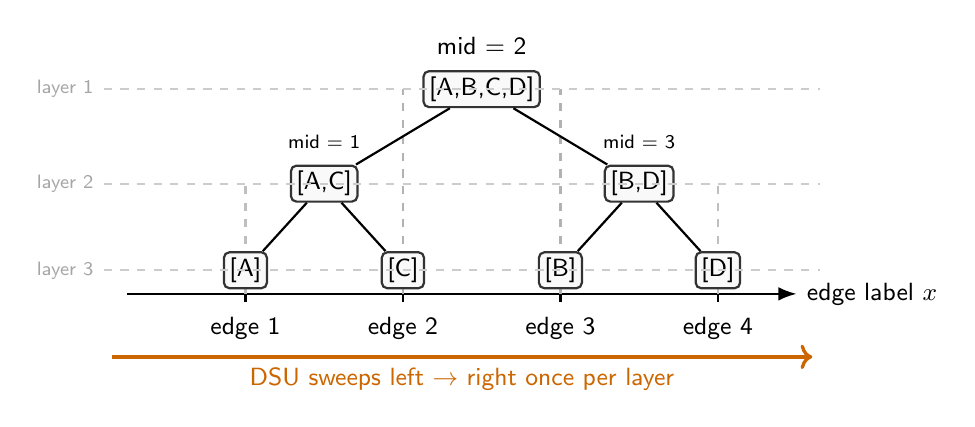
\begin{tikzpicture}[
			thick,
			every node/.style={font=\small},
			interval/.style={rectangle, draw=black!80, rounded corners=2pt, fill=gray!5, inner sep=2pt},
			arrow/.style={->, thick, >=Stealth}
		]

		% Axis with edges (0.5 spacing per edge for proportional look)
		\draw[thick, -Latex] (0,0) -- (8.5,0) node[right] {edge label $x$};
		\foreach \x/\num in {1.5/1,3.5/2,5.5/3,7.5/4}
		\draw (\x,0.1) -- (\x,-0.1) node[below=2pt] {edge \num};

		% Root (layer 1)
		\node[interval] (root) at (4.5,2.6) {[A,B,C,D]};
		\node[above=2pt of root] {\small mid = 2};
		\draw[dashed, gray!60] (3.5,0) -- (3.5,2.6);
		\draw[dashed, gray!60] (5.5,0) -- (5.5,2.6);

		% Children (layer 2)
		\node[interval] (L) at (2.5,1.4) {[A,C]};
		\node[interval] (R) at (6.5,1.4) {[B,D]};
		\draw (root) -- (L);
		\draw (root) -- (R);
		\node[above=2pt of L] {\scriptsize mid = 1};
		\node[above=2pt of R] {\scriptsize mid = 3};
		\draw[dashed, gray!50] (1.5,0) -- (1.5,1.4);
		\draw[dashed, gray!50] (7.5,0) -- (7.5,1.4);

		% Leaves (layer 3)
		\node[interval] (A) at (1.5,0.3) {[A]};
		\node[interval] (C) at (3.5,0.3) {[C]};
		\node[interval] (B) at (5.5,0.3) {[B]};
		\node[interval] (D) at (7.5,0.3) {[D]};
		\draw (L) -- (A);
		\draw (L) -- (C);
		\draw (R) -- (B);
		\draw (R) -- (D);

		% DSU sweep arrow
		\draw[->, very thick, orange!80!black] (-0.2,-0.8) -- (8.7,-0.8)
		node[midway, below, align=center, font=\small]
		{DSU sweeps left $\to$ right once per layer};

		% Layer guides
		\foreach \y/\labeltext in {2.6/layer 1,1.4/layer 2,0.3/layer 3}{
				\draw[dashed, gray!40] (-0.3,\y) -- (8.8,\y);
				\node[left, gray!70, font=\scriptsize] at (-0.3,\y) {\labeltext};
			}

	\end{tikzpicture}
	\caption{Parallel Binary Search with four edges and queries.}
	\label{fig:pbs1}
\end{figure}

In \autoref{fig:pbs1}, we have four queries \(A, B, C, D\).
Each horizontal dashed line represents one \emph{layer} of the parallel binary search —
that is, one complete \emph{left-to-right sweep} of the edge list by the disjoint-set-union (DSU),
adding edges in increasing order of their labels.

At the first layer, all queries check whether using the first two edges
is sufficient to connect their respective vertex pairs.
After one DSU sweep, we find that this range suffices for queries \(A\) and \(C\),
but not for \(B\) and \(D\).

In the second layer, the remaining searches refine their ranges:
queries \(A\) and \(C\) now test whether only the first edge is enough,
while \(B\) and \(D\) test whether the first three edges suffice.
We again perform a single DSU sweep — adding the first edge, checking \(A\) and \(C\),
then adding the second and third edges, and checking \(B\) and \(D\).

\begin{exercise}
	[POI11 Meteors]
\end{exercise}

\section{CDQ}

\begin{tcolorbox}[colback=white, colframe=gray!40, arc=0pt, boxrule=0.5pt, left=10pt, right=10pt, top=8pt, bottom=8pt]
	\centering
	\Large\itshape
	More dimensions!!!
\end{tcolorbox}

\begin{problem}
There exist $N \le 10^5$ points $P_i = (x_i, y_i, z_i) \in \mathbb{Z_+}^3$. We define relation $<$ as follows: $(x, y, z) < (x', y', z') \iff x < x' \land y < y' \land z < z'$. For each $1 \le i \le N$, let $f(i)$ be number of points $1 \le j \le N$ such that $P_j < P_i$. Find $f(i)$ for all $1 \le i \le N$. To save us from the annoying details, assume that all the abscissas are pairwise distinct. This is the 3D partial order problem.
\end{problem}

\textbf{Solution 1: Bashing 2D point add rectangle sum data structure.}
Iterate over the points in increasing order of $x_i$. To find $f(i)$, query the sum of  rectangle $((0, 0), (y_i, z_i))$. Then add one to point $(y_i, z_i)$. Time and space complexity: $O(N \lg^2 N)$. This is fine but has huge constant and memory usage.

\smallskip

\textbf{Solution 2: CDQ.}
Start by sorting and points in increasing order of abscissa. Let's assume $P$ is already sorted as such. We know that $i < j$ is a necessary condition for $P_i < P_j$. This motivates a divide-and-conquer approach. To find the answer for points in $P$, we divide $P$ into left and right part of balanced size. Now for each point in the right part we consider how many points in the left part is less than itself. Once we do that, the left and right part becomes completely isolated and we can solve the two subproblems.

The usual divide-and-conquer process is to \emph{combine} the results of the two subproblems; however, here it is more like \emph{count contribution between two subproblems and divide}. We do not relate the results of two subproblem in any way. Now, to solve the \emph{count contribution} part -- what we shall solve is essentially: given set $A$ and $B$ of points $(y_i, z_i)$ in a cartesian plane. For all points in $B$ (the right part), count the number of points in $A$ which is less than it. This is a standard problem which can be solved by offline processing and one-dimensional Fenwick tree. Time complexity remains $O(N \lg^2 N)$. However, space complexity is merely $O(N)$, for we use one dimensional range-add-range-sum structure here.

Generally, CDQ is highly useful in cutting off one dimension in a geometric process at a cost of a log factor.


\begin{figure}[H]
	\centering

	\tikzset{
		setA/.style={blue, fill=blue!70},
		setB/.style={red, fill=red!80!black},
		projline/.style={dashed, gray!60, thin}
	}

	%--------------------------
	% 3D PLOT (Divide)
	%--------------------------
	\tdplotsetmaincoords{65}{115}
	\begin{tikzpicture}[tdplot_main_coords, scale=0.9]

		% Title placed discreetly
		\node[font=\bfseries, anchor=south west] at (-0.8,6.5,0)
		{1.\ $\mathbb{Z}_+^3$: Divide by $X$};

		% Axes
		\draw[->, thick] (0,0,0)--(6,0,0) node[below right]{$X$};
		\draw[->, thick] (0,0,0)--(0,6,0) node[left]{$Y$};
		\draw[->, thick] (0,0,0)--(0,0,5) node[above]{$Z$};

		% Split plane at X=3
		\filldraw[fill=green!20, draw=green!60!black, opacity=0.25]
		(3,0,0)--(3,6,0)--(3,6,5)--(3,0,5)--cycle;

		% Set A points (blue circles)
		\foreach \x/\y/\z in {1/2/1, 2/4/2, 2/1/3}{
				\shade[setA] (\x,\y,\z) circle (2pt);
				\draw[projline] (\x,\y,\z)--(0,\y,\z);
			}

		% Set B points (red squares)
		\foreach \x/\y/\z in {4/5/4, 5/3/5, 5/2/4}{
				\draw[setB] (\x,\y,\z) rectangle ++(3pt,3pt);
				\draw[projline] (\x,\y,\z)--(0,\y,\z);
			}


	\end{tikzpicture}

	\vspace{2em}

	%--------------------------
	% 2D PLOT (Conquer)
	%--------------------------
	\begin{tikzpicture}[scale=0.9]
		\node[font=\bfseries, anchor=south west] at (9,2)
		{2.\ $\mathbb{Z}_+^2$: 2D Subproblem};

		\draw[gray!20] (0,0) grid (6,6);

		\draw[->, thick] (0,0)--(6.2,0) node[right]{$Y$};
		\draw[->, thick] (0,0)--(0,6.2) node[above]{$Z$};

		% Projected Set A (blue circles)
		\foreach \y/\z in {2/1,4/2,1/3}{
				\shade[setA] (\y,\z) circle (2pt);
			}

		% Projected Set B (red squares)
		\foreach \y/\z in {5/4,3/5,2/4}{
				\draw[setB] (\y,\z) rectangle ++(3pt,3pt);
			}

		% Example dominance region
		\draw[red, dashed, thick] (0,0) rectangle (3,5);
		\node[red, anchor=south east] at (3,5) {\scriptsize $<$ region};

	\end{tikzpicture}

	\caption{CDQ visualization.
		Top: points in $\mathbb{Z}_+^3$ split by $X=c$ (green plane) into two subsets.
		Bottom: projection onto OYZ-plane forming the 2D dominance subproblem.}
\end{figure}


\begin{exercise} [APIO19\_street]
\end{exercise}

\begin{exercise}
	Invent an $O(N \lg ^3N)$ solution to 4D partial order problem.
\end{exercise}




\smallskip

\begin{exercise} [\href{https://darkbzoj.cc/problem/3295}{DarkBzoj3295}] \end{exercise}
\begin{exercise} [\href{https://zerojudge.tw/ShowProblem?problemid=c571}{ZJc571}] \end{exercise}


\section{Minimum Stack -- Minimum Deque}

\begin{tcolorbox}[colback=white, colframe=gray!40, arc=0pt, boxrule=0.5pt, left=10pt, right=10pt, top=8pt, bottom=8pt]
	\centering
	\Large\itshape
	push, pop, getmin
\end{tcolorbox}

Let us design a stack which support these operations: \verb|push(x)| \verb|pop()| \verb|getmin()|. Where \verb|getmin()| returns the minimum element in stack. This can be implemented in same complexity as standard stack. Maintain two stacks $A, B$; on a \verb|push(x)| operation, push $ min(x, B.top)$ -- or $x$ if $B$ is empty -- to $B$ and push x to $A$. On \verb|pop()| operation, do a pop on both $A$ and $B$. On \verb|getmin()| operation, return $B.top$. Let us call this data structure min-stack.

There is a standard technique for implementing a queue with two stacks. Maintain stacks $A$ and $B$. to do an enqueue operation, push to $A$. To dequeue, if $B$ is empty, repeated push the top of $A$ to $B$ then pop $A$, until $A$ is empty. Then return top of B. The amortized time complexity is constant time per operation,  for each element can only get moved from $A$ to $B$ once. The intuition is that $A$ stores some elements from the rear end of the queue, and $B$ stores the remaining elements.

If we use two min-stacks to implement a queue, we achieve a min-queue. Is it possible to get min-deque? Yes, it turns out we can implement an efficient deque with two stacks. It is almost identical to building a queue -- except we only move half the elements to the empty stack instead of the entirety of the other stack. If we want to pop from $B$ and it is empty, move half top of $A$ to it. If we want to pop from $A$ and it is empty, move half top of $B$ to it.
Now, by using min-stacks to build a deque, we achieve efficient amortized min-deque!
\iffalse
	\section{Dynamic Dynamic Programming}

	\emph{No, that is not a typo.}


	Dynamic DP refers to maintaining dynamic programming on tree with update.

	It is often used in problems like maintaining the maximum-weight independent set
	on a tree under dynamic vertex weight updates.

	\textbf{Static baseline.}
	Consider a static DP on a tree where, for each node $u$,
	\[
		f_{u,0} = \sum_{v \in \text{child}(u)} \max(f_{v,0}, f_{v,1}), \qquad
		f_{u,1} = w_u + \sum_{v \in \text{child}(u)} f_{v,0}.
	\]
	Here $f_{u,0}$ and $f_{u,1}$ represent the best results when node $u$
	is excluded or included, respectively.
	If all weights are fixed, this can be computed with a single DFS in $O(N)$ time.

	\textbf{The difficulty.}
	When a node’s weight changes, recomputing the entire DP from the root
	would require rerunning DFS and recalculating all subtree values.
	This takes $O(N)$ per update, which is too slow for up to $10^5$ modifications.

	\textbf{Dynamic maintenance.}
	To avoid full recomputation, we can represent each node’s DP transition
	as a composable algebraic structure — typically a $2 \times 2$
	\emph{max-plus matrix} encoding the relationship between parent and child states.
	For two subtrees $A$ and $B$, their merged contribution can be written as
	\[
		C_{i,j} = \max_k \big(A_{i,k} + B_{k,j}\big).
	\]
	Because this operation is associative, we can use a segment tree
	or heavy-light decomposition to maintain and merge these matrices efficiently.

	\textbf{Implementation idea.}
	Each vertex stores a matrix summarizing how its DP values interact
	with its parent’s inclusion or exclusion.
	Along each heavy path, we maintain a segment tree whose nodes store
	the product (in the max-plus sense) of child matrices.
	When a weight $w_u$ changes, we update $u$’s matrix
	and recompute products along its heavy path.
	The update and query operations both take $O(\log^2 N)$ time.

	\textbf{Summary.}
	Dynamic DP converts local DP transitions into algebraic operations
	that can be merged efficiently.
	By leveraging associativity and hierarchical decomposition,
	it allows DP problems — previously static — to support fast updates and queries.
	This technique generalizes beyond the tree independent-set problem
	to any DP where transitions can be expressed as composable matrices.
\fi


%\section{Chosen Tasks}

%\chapter{Interactive Tasks}
%\chapter{Two-step Tasks}

%\appendix
%\chapter{Appendices}
\iffalse
	\begin{lstlisting}[caption={Solution to JOI14\_Historical with Rollback Mo's}, label={lst:joi14historical}]]
#include<stdio.h>
#include<string.h>
#include<algorithm>

int n,nq,x[100000],cr,bb[100000],xs[100000],freq[100000];
long long ans[100000],mx;
struct QUERY{
    int l,r,i;
    bool operator<(const QUERY&o)const{
        if(bb[l]!=bb[o.l])return l<o.l;
        return r<o.r;
    }
}q[100000];

int main(){
    scanf("%d%d",&n,&nq);
    for(int i=0;i<n;++i)scanf("%d",&x[i]),bb[i]=i/400,xs[i]=x[i];
    std::sort(xs,xs+n);
    for(int i=0;i<n;++i)x[i]=std::lower_bound(xs,xs+n,x[i])-xs;
    for(int i=0;i<nq;++i)scanf("%d%d",&q[i].l,&q[i].r),q[i].i=i,--q[i].l,--q[i].r;
    std::sort(q,q+nq);
    for(int i=0;i<nq;++i){
        auto&[l,r,i_]=q[i];
        if(!i||bb[l]!=bb[q[i-1].l]){ /* starting new block */
            memset(freq,0,sizeof freq); /* resets D */
            cr=l;
            mx=0;
        }
        while(cr<r){
            ++cr;
            if(bb[cr]>bb[l]){
                ++freq[x[cr]];
                if(freq[x[cr]]*1ll*xs[x[cr]]>mx)
                    mx=1ll*freq[x[cr]]*xs[x[cr]];
            }
        }
        long long mx_=mx;
        for(int j=l;j<=cr&&bb[l]==bb[j];++j){
            /*do temporary leftward moves */
            ++freq[x[j]];
            if(freq[x[j]]*1ll*xs[x[j]]>mx_)
                mx_=1ll*freq[x[j]]*xs[x[j]];
        }
        /* rollback those moves */
        for(int j=l;j<=cr&&bb[l]==bb[j];++j)
            --freq[x[j]];
        ans[i_]=mx_;
    }
    for(int i=0;i<nq;++i)printf("%lld\n",ans[i]);
    return 0;
}
\end{lstlisting}

	\begin{lstlisting}[language=C, caption={Dynacon Solution for Codeforces 1217F}, label={lst:cf1217f_dynacon}]
#include <stdio.h>
#include <string.h>
#include <stdlib.h>

#define N 200000
#define Q 200000
#define Q_ (1 << 18)
#define X (1 << 24) /* max(Q * 2, dsu undo stack size) */

int n, m, m_, op[Q], xx[Q], yy[Q]
        , uu[Q << 1], vv[Q << 1], ii[X], jj[X], jj_[X]
        /* ii[], jj[], are used for sorting uu[], vv[] and ii[], jj[], jj_[]  are reused for dsu rollback */
        , occ[Q << 1], start[Q << 1], end[Q << 1] /* prepare() */
        , active[Q << 1]
        , k
        , ff[N] /* counting sort */
        , /* dsu w/ undo */ ds[N], top, last
        , *eh[Q_ << 1], eo[Q_ << 1];

void append(int i, int j) {
    int o = eo[i]++;
    if (! o)
        eh[i] = (int*)malloc(sizeof **eh * 2);
    else if (!(o & (o - 1)))
        eh[i] = (int*)realloc(eh[i], sizeof **eh * o * 2);
    eh[i][o] = j;
}

int ds_find(int i) {
    if (ds[i] < 0)
        return i;
    return ds_find(ds[i]);
}
int ds_unite(int i, int j) {
    i = ds_find(i), j = ds_find(j);
    if (i == j)
        return 0;
    if (ds[i] > ds[j])
        i ^= j, j ^= i, i ^= j;
    ii[top] = i, jj[top] = j; jj_[top] = ds[j]; ++top;
    ds[i] += ds[j];
    ds[j] = i;
    return 1;
}

void ds_undo() {
    int i, j, j_;
    --top;
    i = ii[top], j = jj[top], j_ = jj_[top];
    ds[i] -= j_;
    ds[j]  = j_;
}

int id(int u, int v) {
    int lower, upper, mid;
    lower = -1, upper = k;
    while (upper - lower > 1) {
        mid = lower + (upper - lower) / 2;
        if (uu[mid] > u || (uu[mid] == u && vv[mid] >= v))
            upper = mid;
        else
            lower = mid;
    }
    return upper;
}

void input() {
    memset(ds, -1, sizeof ds);
    scanf("%d%d", &n, &m);
    for (m_ = 1; m_ < m; m_ <<= 1)
        ;

    for(int i = 0; i < m; ++i) {
        scanf("%d%d%d", op + i, xx + i, yy + i);

        if (op[i] == 2)
            continue;

        for (int fakelast = 0; fakelast < 2; ++fakelast, ++k) {
            uu[k] = (xx[i] + fakelast - 1) % n, vv[k] = (yy[i] + fakelast - 1) % n;
            ii[k] = k;
            if (uu[k] > vv[k])
                uu[k] ^= vv[k], vv[k] ^= uu[k], uu[k] ^= vv[k];
        }
    }

    for (int i = 0; i < k; ++i)
        ++ff[vv[i]];
    for (int i = 1; i < n; ++i)
        ff[i] += ff[i - 1];
    for (int i = 0; i < k; ++i)
        jj[--ff[vv[i]]] = i;
    memset(ff, 0, sizeof ff);
    for (int i = 0; i < k; ++i)
        ++ff[uu[i]];
    for (int i = 1; i < n; ++i)
        ff[i] += ff[i - 1];
    for (int i = k - 1; i >= 0; --i)
        ii[--ff[uu[jj[i]]]] = jj[i];

    for (int i = 0; i < k; ++i)
        jj[i] = uu[ii[i]];
    memcpy(uu, jj, sizeof uu);
    for (int i = 0; i < k; ++i)
        jj[i] = vv[ii[i]];
    memcpy(vv, jj, sizeof vv);
}

void putedge(int id, int l, int r) {
    if (l + 1 >= r)
        return;

    l += m_;
    r += m_;
    for (; l ^ r ^ 1; l >>= 1, r >>= 1) {
        if (l & 1 ^ 1)
            append(l ^ 1, id);
        if (r & 1)
            append(r ^ 1, id);
    }
}

void prepare() {
    for (int i = 0; i < k; ++i)
        ++end[id(uu[i], vv[i])];

    for (int l = 0, i = 0; i < k; ++i)
        start[i] = l, l += end[i], end[i] = start[i];

    for (int ru, rv, i = 0; i < m; ++i) {
        if (op[i] == 2)
            continue;

        for (int fakelast = 0; fakelast < 2; ++fakelast) {
            ru = (xx[i] + fakelast - 1) % n, rv = (yy[i] + fakelast - 1) % n;
            if (ru > rv)
                ru ^= rv, rv ^= ru, ru ^= rv;
            occ[end[id(ru, rv)]++] = i;
        }
    }

    for (int last_put, i = 0; i < k; ++i) {
        if (start[i] == end[i])
            continue;

        last_put = occ[start[i]];
        for (int j = start[i] + 1; j ^ end[i]; ++j)
            putedge(i, last_put, occ[j]), last_put = occ[j];

        putedge(i, last_put, m);
    }
}

void dnc(int v, int l, int r) {
    if (l >= m)
        return;

    int inserted = 0;

    for (int j, i = 0; i < eo[v]; ++i)
        if (active[j = eh[v][i]])
            inserted += ds_unite(uu[j], vv[j]);

    if (l + 1 == r) {
        int ru, rv;
        ru = (xx[l] + last - 1) % n, rv = (yy[l] + last - 1) % n;
        if (ru > rv)
            ru ^= rv, rv ^= ru, ru ^= rv;

        if (op[l] == 2) {
            last = ds_find(ru) == ds_find(rv);
            putchar(last + '0');
        } else
            active[id(ru, rv)] ^= 1;
    } else {
        int md = (l + r) / 2;
        dnc(v << 1, l, md);
        dnc(v << 1 | 1, md, r);
    }

    while (inserted--)
        ds_undo();
}

int main(){
    input();
    prepare();

    dnc(1, 0, m_);
    return 0;
}
\end{lstlisting}

	\begin{lstlisting}[language=C, caption={Edge centroid decomp. TIMUS2085},
label={lst:timus2085}]
#include<stdio.h>
#include<algorithm>
#include<random>
using namespace std;
random_device rd;
mt19937_64 rng(rd());

#define M 100000
#define N_ (N*2+1)
#define N 100000

using u64=unsigned long long;
int rt,n,m,hd[N],e[N_],Ln[N_],ii,diff,midedge,kil[N_],sz[N],o[N],p;
u64 qwq[M+1],val[N],dis[N],sum;

void add(int u,int v){ ++ii; e[ii]=v;Ln[ii]=hd[u]; hd[u]=ii; }
void dfs0(int u,int p){
	sz[u]=1;
	for(int j=hd[u];j;j=Ln[j])if(!kil[j]&&e[j]!=p){
		dfs0(e[j],u),sz[u]+=sz[e[j]];
	}
}
void dfs1(int u,int code){
	int x_=abs(sz[u]-(sz[rt]-sz[u]));
	if(x_<diff)diff=x_,midedge=code;
	for(int j=hd[u];j;j=Ln[j])if(!kil[j]&&(j^code^1))dfs1(e[j],j);
}

void answer(int i,int j){
	printf("%d %d\n",i+1,j+1);
	exit(0);
}
void dfs2(int u,int code){
	dis[u]+=val[u];
	if(dis[u]==sum){
		answer(rt,u);
	}
	o[p++]=u;
	for(int j=hd[u];j;j=Ln[j])if(!kil[j]&&(j^code^1)) dis[e[j]]=dis[u],dfs2(e[j],j);
}

void dfs3(int u,int code,u64 d){
	d+=val[u];
	int x=0;
	for(int j=(1<<20);j;j>>=1)
		if(j+x<p&&dis[o[x+j]]<=sum-d)x+=j;
	if(dis[o[x]]==sum-d)answer(o[x],u);
	for(int j=hd[u];j;j=Ln[j])if(!kil[j]&&(j^code^1)) dfs3(e[j],j,d);
}

void DECOM(int u){
	dfs0(u,-1);
	diff=1900000;rt=u;dfs1(u,0);

	if(midedge){
		int x=e[midedge],y=e[midedge^1];
		kil[midedge]=kil[midedge^1]=1;
		rt=x;dis[x]=p=0;dfs2(x,0);std::sort(o,o+p,[](int i,int j){return dis[i]<dis[j];});dfs3(y,0,0);
		rt=y;dis[y]=p=0;dfs2(y,0);std::sort(o,o+p,[](int i,int j){return dis[i]<dis[j];});dfs3(x,0,0);

		DECOM(x),DECOM(y);
	}
}

int main(){
	ii=1;

	scanf("%d%d",&n,&m);
	for(int i=1;i<=m;++i)qwq[i]=rng(),sum+=qwq[i];
	for(int u,v,i=1;i<n;++i){
		scanf("%d%d",&u,&v),--u,--v;
		add(u,v),add(v,u);
	}
	for(int sz,w,i=0;i<n;++i){
		scanf("%d",&sz);
		while(sz--)scanf("%d",&w),val[i]+=qwq[w];
	}

	DECOM(0);
	puts("No solution");

	return 0;
}
\end{lstlisting}
\fi
\clearpage
\phantomsection
\addcontentsline{toc}{chapter}{References}

% Include all entries from oi-book.bib, even if uncited
\nocite{*}

\bibliographystyle{abbrvnat} % or plainnat, alpha, etc.
\bibliography{book}

\end{document}
